\documentclass{book}
\usepackage[a4paper,top=2.5cm,bottom=2.5cm,left=2.5cm,right=2.5cm]{geometry}
\usepackage{makeidx}
\usepackage{natbib}
\usepackage{graphicx}
\usepackage{multicol}
\usepackage{float}
\usepackage{listings}
\usepackage{color}
\usepackage{ifthen}
\usepackage[table]{xcolor}
\usepackage{textcomp}
\usepackage{alltt}
\usepackage{ifpdf}
\ifpdf
\usepackage[pdftex,
            pagebackref=true,
            colorlinks=true,
            linkcolor=blue,
            unicode
           ]{hyperref}
\else
\usepackage[ps2pdf,
            pagebackref=true,
            colorlinks=true,
            linkcolor=blue,
            unicode
           ]{hyperref}
\usepackage{pspicture}
\fi
\usepackage[utf8]{inputenc}
\usepackage{mathptmx}
\usepackage[scaled=.90]{helvet}
\usepackage{courier}
\usepackage{sectsty}
\usepackage[titles]{tocloft}
\usepackage{doxygen}
\lstset{language=C++,inputencoding=utf8,basicstyle=\footnotesize,breaklines=true,breakatwhitespace=true,tabsize=8,numbers=left }
\makeindex
\setcounter{tocdepth}{3}
\renewcommand{\footrulewidth}{0.4pt}
\renewcommand{\familydefault}{\sfdefault}
\hfuzz=15pt
\setlength{\emergencystretch}{15pt}
\hbadness=750
\tolerance=750
\begin{document}
\hypersetup{pageanchor=false,citecolor=blue}
\begin{titlepage}
\vspace*{7cm}
\begin{center}
{\Large Rage\-Pixel }\\
\vspace*{1cm}
{\large Generated by Doxygen 1.8.0}\\
\vspace*{0.5cm}
{\small Tue May 8 2012 20:54:21}\\
\end{center}
\end{titlepage}
\clearemptydoublepage
\pagenumbering{roman}
\tableofcontents
\clearemptydoublepage
\pagenumbering{arabic}
\hypersetup{pageanchor=true,citecolor=blue}
\chapter{Class Index}
\section{Class Hierarchy}
This inheritance list is sorted roughly, but not completely, alphabetically\-:\begin{DoxyCompactList}
\item \contentsline{section}{I\-Rage\-Pixel}{\pageref{interface_i_rage_pixel}}{}
\begin{DoxyCompactList}
\item \contentsline{section}{Rage\-Pixel\-Sprite}{\pageref{class_rage_pixel_sprite}}{}
\end{DoxyCompactList}
\item \contentsline{section}{Rage\-Pixel\-Animation}{\pageref{class_rage_pixel_animation}}{}
\item \contentsline{section}{Rage\-Pixel\-Anim\-Strip\-G\-U\-I}{\pageref{class_rage_pixel_anim_strip_g_u_i}}{}
\item \contentsline{section}{Rage\-Pixel\-Bitmap}{\pageref{class_rage_pixel_bitmap}}{}
\item \contentsline{section}{Rage\-Pixel\-Camera}{\pageref{class_rage_pixel_camera}}{}
\item \contentsline{section}{Rage\-Pixel\-Camera\-Editor}{\pageref{class_rage_pixel_camera_editor}}{}
\item \contentsline{section}{Rage\-Pixel\-Cell}{\pageref{class_rage_pixel_cell}}{}
\item \contentsline{section}{Rage\-Pixel\-Color\-Picker\-G\-U\-I}{\pageref{class_rage_pixel_color_picker_g_u_i}}{}
\item \contentsline{section}{Rage\-Pixel\-H\-S\-B\-Color}{\pageref{struct_rage_pixel_h_s_b_color}}{}
\item \contentsline{section}{Rage\-Pixel\-Palette\-G\-U\-I}{\pageref{class_rage_pixel_palette_g_u_i}}{}
\item \contentsline{section}{Rage\-Pixel\-Row}{\pageref{class_rage_pixel_row}}{}
\item \contentsline{section}{Rage\-Pixel\-Settings}{\pageref{class_rage_pixel_settings}}{}
\item \contentsline{section}{Rage\-Pixel\-Sprite\-Editor}{\pageref{class_rage_pixel_sprite_editor}}{}
\item \contentsline{section}{Rage\-Pixel\-Sprite\-Sheet}{\pageref{class_rage_pixel_sprite_sheet}}{}
\item \contentsline{section}{Rage\-Pixel\-Sprite\-Sheet\-Editor\-Window}{\pageref{class_rage_pixel_sprite_sheet_editor_window}}{}
\item \contentsline{section}{Rage\-Pixel\-Sprite\-Sheet\-G\-U\-I}{\pageref{class_rage_pixel_sprite_sheet_g_u_i}}{}
\item \contentsline{section}{Rage\-Pixel\-Texel}{\pageref{class_rage_pixel_texel}}{}
\item \contentsline{section}{Rage\-Pixel\-Texel\-Rect}{\pageref{class_rage_pixel_texel_rect}}{}
\item \contentsline{section}{Rage\-Pixel\-Transform\-Inspector}{\pageref{class_rage_pixel_transform_inspector}}{}
\end{DoxyCompactList}

\chapter{Class Index}
\section{Class List}
Here are the classes, structs, unions and interfaces with brief descriptions\-:\begin{DoxyCompactList}
\item\contentsline{section}{\hyperlink{interface_i_rage_pixel}{I\-Rage\-Pixel} }{\pageref{interface_i_rage_pixel}}{}
\item\contentsline{section}{\hyperlink{class_rage_pixel_animation}{Rage\-Pixel\-Animation} }{\pageref{class_rage_pixel_animation}}{}
\item\contentsline{section}{\hyperlink{class_rage_pixel_anim_strip_g_u_i}{Rage\-Pixel\-Anim\-Strip\-G\-U\-I} }{\pageref{class_rage_pixel_anim_strip_g_u_i}}{}
\item\contentsline{section}{\hyperlink{class_rage_pixel_bitmap}{Rage\-Pixel\-Bitmap} }{\pageref{class_rage_pixel_bitmap}}{}
\item\contentsline{section}{\hyperlink{class_rage_pixel_camera}{Rage\-Pixel\-Camera} }{\pageref{class_rage_pixel_camera}}{}
\item\contentsline{section}{\hyperlink{class_rage_pixel_camera_editor}{Rage\-Pixel\-Camera\-Editor} }{\pageref{class_rage_pixel_camera_editor}}{}
\item\contentsline{section}{\hyperlink{class_rage_pixel_cell}{Rage\-Pixel\-Cell} }{\pageref{class_rage_pixel_cell}}{}
\item\contentsline{section}{\hyperlink{class_rage_pixel_color_picker_g_u_i}{Rage\-Pixel\-Color\-Picker\-G\-U\-I} }{\pageref{class_rage_pixel_color_picker_g_u_i}}{}
\item\contentsline{section}{\hyperlink{struct_rage_pixel_h_s_b_color}{Rage\-Pixel\-H\-S\-B\-Color} }{\pageref{struct_rage_pixel_h_s_b_color}}{}
\item\contentsline{section}{\hyperlink{class_rage_pixel_palette_g_u_i}{Rage\-Pixel\-Palette\-G\-U\-I} }{\pageref{class_rage_pixel_palette_g_u_i}}{}
\item\contentsline{section}{\hyperlink{class_rage_pixel_row}{Rage\-Pixel\-Row} }{\pageref{class_rage_pixel_row}}{}
\item\contentsline{section}{\hyperlink{class_rage_pixel_settings}{Rage\-Pixel\-Settings} }{\pageref{class_rage_pixel_settings}}{}
\item\contentsline{section}{\hyperlink{class_rage_pixel_sprite}{Rage\-Pixel\-Sprite} }{\pageref{class_rage_pixel_sprite}}{}
\item\contentsline{section}{\hyperlink{class_rage_pixel_sprite_editor}{Rage\-Pixel\-Sprite\-Editor} }{\pageref{class_rage_pixel_sprite_editor}}{}
\item\contentsline{section}{\hyperlink{class_rage_pixel_sprite_sheet}{Rage\-Pixel\-Sprite\-Sheet} }{\pageref{class_rage_pixel_sprite_sheet}}{}
\item\contentsline{section}{\hyperlink{class_rage_pixel_sprite_sheet_editor_window}{Rage\-Pixel\-Sprite\-Sheet\-Editor\-Window} }{\pageref{class_rage_pixel_sprite_sheet_editor_window}}{}
\item\contentsline{section}{\hyperlink{class_rage_pixel_sprite_sheet_g_u_i}{Rage\-Pixel\-Sprite\-Sheet\-G\-U\-I} }{\pageref{class_rage_pixel_sprite_sheet_g_u_i}}{}
\item\contentsline{section}{\hyperlink{class_rage_pixel_texel}{Rage\-Pixel\-Texel} }{\pageref{class_rage_pixel_texel}}{}
\item\contentsline{section}{\hyperlink{class_rage_pixel_texel_rect}{Rage\-Pixel\-Texel\-Rect} }{\pageref{class_rage_pixel_texel_rect}}{}
\item\contentsline{section}{\hyperlink{class_rage_pixel_transform_inspector}{Rage\-Pixel\-Transform\-Inspector} }{\pageref{class_rage_pixel_transform_inspector}}{}
\end{DoxyCompactList}

\chapter{Class Documentation}
\hypertarget{interface_i_rage_pixel}{\section{I\-Rage\-Pixel Interface Reference}
\label{interface_i_rage_pixel}\index{I\-Rage\-Pixel@{I\-Rage\-Pixel}}
}


Inheritance diagram for I\-Rage\-Pixel\-:
\nopagebreak
\begin{figure}[H]
\begin{center}
\leavevmode
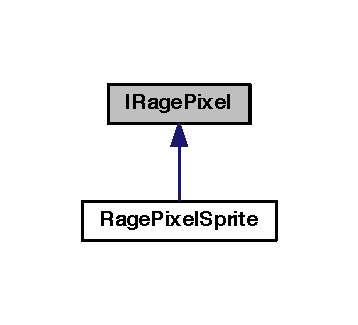
\includegraphics[width=172pt]{interface_i_rage_pixel__inherit__graph}
\end{center}
\end{figure}
\subsection*{Public Member Functions}
\begin{DoxyCompactItemize}
\item 
\hypertarget{interface_i_rage_pixel_aa84818acdc7e9d2ef80230323d1fc050}{void {\bfseries Set\-Sprite} (string name)}\label{interface_i_rage_pixel_aa84818acdc7e9d2ef80230323d1fc050}

\item 
\hypertarget{interface_i_rage_pixel_a47e40c8dbd24bf9ab622ac7043073035}{void {\bfseries Set\-Sprite} (string name, int frame\-Index)}\label{interface_i_rage_pixel_a47e40c8dbd24bf9ab622ac7043073035}

\item 
\hypertarget{interface_i_rage_pixel_a0879278adb76f52123970c44ebac453b}{void {\bfseries Play\-Animation} ()}\label{interface_i_rage_pixel_a0879278adb76f52123970c44ebac453b}

\item 
\hypertarget{interface_i_rage_pixel_a9d87548ffed46340c0f6d711b7c59991}{void {\bfseries Play\-Animation} (bool force\-Restart)}\label{interface_i_rage_pixel_a9d87548ffed46340c0f6d711b7c59991}

\item 
\hypertarget{interface_i_rage_pixel_a4061820f2995a1eace11719a6c32e173}{void {\bfseries Play\-Animation} (bool force\-Restart, int range\-Min\-Index, int range\-Max\-Index, int priority=0)}\label{interface_i_rage_pixel_a4061820f2995a1eace11719a6c32e173}

\item 
\hypertarget{interface_i_rage_pixel_a107544fa8c2f3f4a2913a39926253dbd}{void {\bfseries Play\-Animation} (bool force\-Restart, int\mbox{[}$\,$\mbox{]} frames, int pri=0)}\label{interface_i_rage_pixel_a107544fa8c2f3f4a2913a39926253dbd}

\item 
\hypertarget{interface_i_rage_pixel_a57974dc9e9794eda716f2c52471f3a5b}{void {\bfseries Play\-Animation} (bool force\-Restart, Rage\-Pixel\-Sprite.\-Animation\-Mode anim\-Mode, int range\-Min\-Index, int range\-Max\-Index, int priority=0)}\label{interface_i_rage_pixel_a57974dc9e9794eda716f2c52471f3a5b}

\item 
\hypertarget{interface_i_rage_pixel_a38386cb8b12865b0754fb5e0d326e869}{void {\bfseries Play\-Animation} (bool force\-Restart, Rage\-Pixel\-Sprite.\-Animation\-Mode anim\-Mode, int\mbox{[}$\,$\mbox{]} frames, int priority=0)}\label{interface_i_rage_pixel_a38386cb8b12865b0754fb5e0d326e869}

\item 
\hypertarget{interface_i_rage_pixel_a238311c1825d86210ed9f479f144c19c}{void {\bfseries Play\-Named\-Animation} (string name, int priority=0)}\label{interface_i_rage_pixel_a238311c1825d86210ed9f479f144c19c}

\item 
\hypertarget{interface_i_rage_pixel_a7b51f0c20206c632592733bb20c25989}{void {\bfseries Play\-Named\-Animation} (string name, bool force\-Restart, int priority=0)}\label{interface_i_rage_pixel_a7b51f0c20206c632592733bb20c25989}

\item 
\hypertarget{interface_i_rage_pixel_ad70e7b7b47ca30e5d292480ed722ab15}{void {\bfseries Play\-Named\-Animation} (string name, bool force\-Restart, float delay\-First\-Frame, int priority=0)}\label{interface_i_rage_pixel_ad70e7b7b47ca30e5d292480ed722ab15}

\item 
\hypertarget{interface_i_rage_pixel_a0d6fc45f3299498cfd21301904bea7e0}{bool {\bfseries Has\-Named\-Animation} (string name)}\label{interface_i_rage_pixel_a0d6fc45f3299498cfd21301904bea7e0}

\item 
\hypertarget{interface_i_rage_pixel_a48ca7f62bcce0f0d25dfce3da97c7155}{bool {\bfseries is\-Playing} ()}\label{interface_i_rage_pixel_a48ca7f62bcce0f0d25dfce3da97c7155}

\item 
\hypertarget{interface_i_rage_pixel_aa0e42c7b01a5c996d88e3b439d57362a}{void {\bfseries Stop\-Animation} ()}\label{interface_i_rage_pixel_aa0e42c7b01a5c996d88e3b439d57362a}

\item 
\hypertarget{interface_i_rage_pixel_a272cfec9fa3b80588c59e7381e37b2f6}{int {\bfseries Get\-Size\-X} ()}\label{interface_i_rage_pixel_a272cfec9fa3b80588c59e7381e37b2f6}

\item 
\hypertarget{interface_i_rage_pixel_a57f635a748ceea4222b0891a0b82d139}{int {\bfseries Get\-Size\-Y} ()}\label{interface_i_rage_pixel_a57f635a748ceea4222b0891a0b82d139}

\item 
\hypertarget{interface_i_rage_pixel_a9fb4204bcc05381c43ab2a4ea0eefbc0}{void {\bfseries Set\-Size} (int width, int height)}\label{interface_i_rage_pixel_a9fb4204bcc05381c43ab2a4ea0eefbc0}

\item 
\hypertarget{interface_i_rage_pixel_a66d97dacd871c546af228bd569194a5b}{Rect {\bfseries Get\-Rect} ()}\label{interface_i_rage_pixel_a66d97dacd871c546af228bd569194a5b}

\item 
\hypertarget{interface_i_rage_pixel_a6bde32575fefc327f9b1df98773fa438}{void {\bfseries Set\-Horizontal\-Flip} (bool value)}\label{interface_i_rage_pixel_a6bde32575fefc327f9b1df98773fa438}

\item 
\hypertarget{interface_i_rage_pixel_a140c7a6f5fdbfd25132bb6ffb6becd2f}{void {\bfseries Set\-Vertical\-Flip} (bool value)}\label{interface_i_rage_pixel_a140c7a6f5fdbfd25132bb6ffb6becd2f}

\item 
\hypertarget{interface_i_rage_pixel_ab446f50e5fe3aeb3713ac82dce738431}{void {\bfseries Set\-Tint\-Color} (Color color)}\label{interface_i_rage_pixel_ab446f50e5fe3aeb3713ac82dce738431}

\end{DoxyCompactItemize}


\subsection{Detailed Description}


Definition at line 4 of file I\-Rage\-Pixel.\-cs.



The documentation for this interface was generated from the following file\-:\begin{DoxyCompactItemize}
\item 
assets/\-Rage\-Pixel/\-Rage\-Pixel\-Mono\-Develop/code/I\-Rage\-Pixel.\-cs\end{DoxyCompactItemize}

\hypertarget{class_rage_pixel_animation}{\section{Rage\-Pixel\-Animation Class Reference}
\label{class_rage_pixel_animation}\index{Rage\-Pixel\-Animation@{Rage\-Pixel\-Animation}}
}


Collaboration diagram for Rage\-Pixel\-Animation\-:
\nopagebreak
\begin{figure}[H]
\begin{center}
\leavevmode
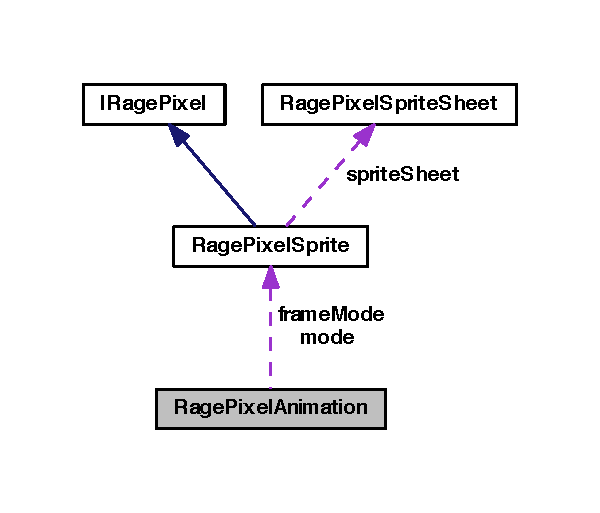
\includegraphics[width=288pt]{class_rage_pixel_animation__coll__graph}
\end{center}
\end{figure}
\subsection*{Public Member Functions}
\begin{DoxyCompactItemize}
\item 
\hypertarget{class_rage_pixel_animation_a71e2dff56a081d5e88439e6484831aab}{\hyperlink{class_rage_pixel_animation}{Rage\-Pixel\-Animation} {\bfseries Clone} ()}\label{class_rage_pixel_animation_a71e2dff56a081d5e88439e6484831aab}

\end{DoxyCompactItemize}
\subsection*{Public Attributes}
\begin{DoxyCompactItemize}
\item 
\hypertarget{class_rage_pixel_animation_a4038df9daf7a413b5646cee41b182911}{string {\bfseries name}}\label{class_rage_pixel_animation_a4038df9daf7a413b5646cee41b182911}

\item 
\hypertarget{class_rage_pixel_animation_a24da08f4d3a777db979e068e8f115d8a}{Rage\-Pixel\-Sprite.\-Animation\-Mode {\bfseries mode} = 0}\label{class_rage_pixel_animation_a24da08f4d3a777db979e068e8f115d8a}

\item 
\hypertarget{class_rage_pixel_animation_a64485d447bc004c4ba8eade67219680c}{Rage\-Pixel\-Sprite.\-Frame\-Mode {\bfseries frame\-Mode} = 0}\label{class_rage_pixel_animation_a64485d447bc004c4ba8eade67219680c}

\item 
\hypertarget{class_rage_pixel_animation_a7e933354127c1d51515ff8ee568a1cdd}{int {\bfseries start\-Index}}\label{class_rage_pixel_animation_a7e933354127c1d51515ff8ee568a1cdd}

\item 
\hypertarget{class_rage_pixel_animation_a9502946898c421494831e3cb8cb7981d}{int {\bfseries end\-Index}}\label{class_rage_pixel_animation_a9502946898c421494831e3cb8cb7981d}

\item 
\hypertarget{class_rage_pixel_animation_a1cf893f3f61d68ca236b4347088f3cde}{int\mbox{[}$\,$\mbox{]} {\bfseries frames}}\label{class_rage_pixel_animation_a1cf893f3f61d68ca236b4347088f3cde}

\end{DoxyCompactItemize}


\subsection{Detailed Description}


Definition at line 5 of file Rage\-Pixel\-Animation.\-cs.



The documentation for this class was generated from the following file\-:\begin{DoxyCompactItemize}
\item 
assets/\-Rage\-Pixel/\-Rage\-Pixel\-Mono\-Develop/code/Rage\-Pixel\-Animation.\-cs\end{DoxyCompactItemize}

\hypertarget{class_rage_pixel_anim_strip_g_u_i}{\section{Rage\-Pixel\-Anim\-Strip\-G\-U\-I Class Reference}
\label{class_rage_pixel_anim_strip_g_u_i}\index{Rage\-Pixel\-Anim\-Strip\-G\-U\-I@{Rage\-Pixel\-Anim\-Strip\-G\-U\-I}}
}


Collaboration diagram for Rage\-Pixel\-Anim\-Strip\-G\-U\-I\-:
\nopagebreak
\begin{figure}[H]
\begin{center}
\leavevmode
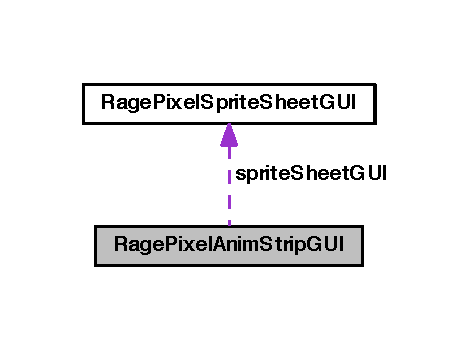
\includegraphics[width=227pt]{class_rage_pixel_anim_strip_g_u_i__coll__graph}
\end{center}
\end{figure}
\subsection*{Public Member Functions}
\begin{DoxyCompactItemize}
\item 
\hypertarget{class_rage_pixel_anim_strip_g_u_i_a106c55c93cc4e2510406bb7663f86b7a}{{\bfseries Rage\-Pixel\-Anim\-Strip\-G\-U\-I} (\hyperlink{class_rage_pixel_sprite_sheet_g_u_i}{Rage\-Pixel\-Sprite\-Sheet\-G\-U\-I} sprite\-Sheet\-G\-U\-I)}\label{class_rage_pixel_anim_strip_g_u_i_a106c55c93cc4e2510406bb7663f86b7a}

\item 
\hypertarget{class_rage_pixel_anim_strip_g_u_i_aea61c5446d6b76f23435c0641e161dc4}{bool {\bfseries size\-Is\-Dirty} (int new\-Max\-Width)}\label{class_rage_pixel_anim_strip_g_u_i_aea61c5446d6b76f23435c0641e161dc4}

\item 
\hypertarget{class_rage_pixel_anim_strip_g_u_i_a3bf00838edd505b58ec33bd925e18456}{void {\bfseries Create\-Texture\-Instance} ()}\label{class_rage_pixel_anim_strip_g_u_i_a3bf00838edd505b58ec33bd925e18456}

\item 
\hypertarget{class_rage_pixel_anim_strip_g_u_i_a585fb26b714d0c21cdad454dda010613}{void {\bfseries Refresh} ()}\label{class_rage_pixel_anim_strip_g_u_i_a585fb26b714d0c21cdad454dda010613}

\item 
\hypertarget{class_rage_pixel_anim_strip_g_u_i_a70d70bb0fe4ca83c72df97b2d83aede1}{int {\bfseries Get\-Row\-Index} (int local\-X, int local\-Y)}\label{class_rage_pixel_anim_strip_g_u_i_a70d70bb0fe4ca83c72df97b2d83aede1}

\item 
\hypertarget{class_rage_pixel_anim_strip_g_u_i_a50b2400b3aaa01c2b5ee9cd3976d3645}{bool {\bfseries Handle\-G\-U\-I\-Event} (Event ev)}\label{class_rage_pixel_anim_strip_g_u_i_a50b2400b3aaa01c2b5ee9cd3976d3645}

\item 
\hypertarget{class_rage_pixel_anim_strip_g_u_i_ad52a0f900dc0344e4d5302b5b32cb429}{void {\bfseries Clean\-Exit} ()}\label{class_rage_pixel_anim_strip_g_u_i_ad52a0f900dc0344e4d5302b5b32cb429}

\end{DoxyCompactItemize}
\subsection*{Public Attributes}
\begin{DoxyCompactItemize}
\item 
Color {\bfseries background\-Color}
\item 
\hypertarget{class_rage_pixel_anim_strip_g_u_i_ab1b522fdd7b0087c4ab464920e52d4aa}{\hyperlink{class_rage_pixel_sprite_sheet_g_u_i}{Rage\-Pixel\-Sprite\-Sheet\-G\-U\-I} {\bfseries sprite\-Sheet\-G\-U\-I}}\label{class_rage_pixel_anim_strip_g_u_i_ab1b522fdd7b0087c4ab464920e52d4aa}

\item 
\hypertarget{class_rage_pixel_anim_strip_g_u_i_ab22e679229cfefcc46ca470488d49c00}{bool {\bfseries visible} = false}\label{class_rage_pixel_anim_strip_g_u_i_ab22e679229cfefcc46ca470488d49c00}

\item 
\hypertarget{class_rage_pixel_anim_strip_g_u_i_a07dea9294c49511cd9f5b5bbfa7a97ae}{bool {\bfseries is\-Dirty} = false}\label{class_rage_pixel_anim_strip_g_u_i_a07dea9294c49511cd9f5b5bbfa7a97ae}

\item 
\hypertarget{class_rage_pixel_anim_strip_g_u_i_a41ebf22267cee30d07a189afe5f1bac9}{int {\bfseries drag\-Target\-Index} = -\/1}\label{class_rage_pixel_anim_strip_g_u_i_a41ebf22267cee30d07a189afe5f1bac9}

\item 
\hypertarget{class_rage_pixel_anim_strip_g_u_i_a9bf6cc8f7e5b00cfbaa2904d37738135}{int {\bfseries position\-X}}\label{class_rage_pixel_anim_strip_g_u_i_a9bf6cc8f7e5b00cfbaa2904d37738135}

\item 
\hypertarget{class_rage_pixel_anim_strip_g_u_i_aec7b93b963494268178de364beebcaf9}{int {\bfseries position\-Y}}\label{class_rage_pixel_anim_strip_g_u_i_aec7b93b963494268178de364beebcaf9}

\end{DoxyCompactItemize}
\subsection*{Properties}
\begin{DoxyCompactItemize}
\item 
\hypertarget{class_rage_pixel_anim_strip_g_u_i_a887d7b6a32797bdb359b2eda2f44aa7c}{Rect {\bfseries bounds}\hspace{0.3cm}{\ttfamily  \mbox{[}get\mbox{]}}}\label{class_rage_pixel_anim_strip_g_u_i_a887d7b6a32797bdb359b2eda2f44aa7c}

\item 
\hypertarget{class_rage_pixel_anim_strip_g_u_i_ae63d3bb53b61f3afb329749d951cc1a4}{Texture2\-D {\bfseries anim\-Strip\-Texture}\hspace{0.3cm}{\ttfamily  \mbox{[}get\mbox{]}}}\label{class_rage_pixel_anim_strip_g_u_i_ae63d3bb53b61f3afb329749d951cc1a4}

\item 
\hypertarget{class_rage_pixel_anim_strip_g_u_i_ac698c6df96bef0d58d6202ebacb17bfa}{\hyperlink{class_rage_pixel_sprite_sheet}{Rage\-Pixel\-Sprite\-Sheet} {\bfseries sprite\-Sheet}\hspace{0.3cm}{\ttfamily  \mbox{[}get\mbox{]}}}\label{class_rage_pixel_anim_strip_g_u_i_ac698c6df96bef0d58d6202ebacb17bfa}

\item 
\hypertarget{class_rage_pixel_anim_strip_g_u_i_a77d89f7c9926e1b08f758c17e5fdbd26}{int {\bfseries current\-Row\-Key}\hspace{0.3cm}{\ttfamily  \mbox{[}get\mbox{]}}}\label{class_rage_pixel_anim_strip_g_u_i_a77d89f7c9926e1b08f758c17e5fdbd26}

\item 
\hypertarget{class_rage_pixel_anim_strip_g_u_i_ab6eb40c0eda97a612b7e2f1d5ba7f8aa}{int {\bfseries current\-Cell\-Key}\hspace{0.3cm}{\ttfamily  \mbox{[}get, set\mbox{]}}}\label{class_rage_pixel_anim_strip_g_u_i_ab6eb40c0eda97a612b7e2f1d5ba7f8aa}

\item 
\hypertarget{class_rage_pixel_anim_strip_g_u_i_a0feef9c8f099c6a2aa2c47192bf9140a}{int {\bfseries max\-Width}\hspace{0.3cm}{\ttfamily  \mbox{[}get, set\mbox{]}}}\label{class_rage_pixel_anim_strip_g_u_i_a0feef9c8f099c6a2aa2c47192bf9140a}

\item 
\hypertarget{class_rage_pixel_anim_strip_g_u_i_a4f3bb27a39e6e484c7dacca2d7af709b}{int {\bfseries thumbnail\-Size}\hspace{0.3cm}{\ttfamily  \mbox{[}get\mbox{]}}}\label{class_rage_pixel_anim_strip_g_u_i_a4f3bb27a39e6e484c7dacca2d7af709b}

\item 
\hypertarget{class_rage_pixel_anim_strip_g_u_i_aa32986e2ac209b1906969a1332074653}{int {\bfseries table\-Width}\hspace{0.3cm}{\ttfamily  \mbox{[}get\mbox{]}}}\label{class_rage_pixel_anim_strip_g_u_i_aa32986e2ac209b1906969a1332074653}

\item 
\hypertarget{class_rage_pixel_anim_strip_g_u_i_afbb5786f7e35edbbeb2871174425f73e}{int {\bfseries table\-Height}\hspace{0.3cm}{\ttfamily  \mbox{[}get\mbox{]}}}\label{class_rage_pixel_anim_strip_g_u_i_afbb5786f7e35edbbeb2871174425f73e}

\item 
\hypertarget{class_rage_pixel_anim_strip_g_u_i_a3372d9b2be5cdcb3ae9b1c30fbf6f669}{int {\bfseries pixel\-Width}\hspace{0.3cm}{\ttfamily  \mbox{[}get, set\mbox{]}}}\label{class_rage_pixel_anim_strip_g_u_i_a3372d9b2be5cdcb3ae9b1c30fbf6f669}

\item 
\hypertarget{class_rage_pixel_anim_strip_g_u_i_acc4978a7d489c80c9864839184fcb457}{int {\bfseries pixel\-Height}\hspace{0.3cm}{\ttfamily  \mbox{[}get, set\mbox{]}}}\label{class_rage_pixel_anim_strip_g_u_i_acc4978a7d489c80c9864839184fcb457}

\end{DoxyCompactItemize}


\subsection{Detailed Description}


Definition at line 5 of file Rage\-Pixel\-Anim\-Strip\-G\-U\-I.\-cs.



\subsection{Member Data Documentation}
\hypertarget{class_rage_pixel_anim_strip_g_u_i_a32855ec0e134a8626a339c54d4aa07b9}{\index{Rage\-Pixel\-Anim\-Strip\-G\-U\-I@{Rage\-Pixel\-Anim\-Strip\-G\-U\-I}!background\-Color@{background\-Color}}
\index{background\-Color@{background\-Color}!RagePixelAnimStripGUI@{Rage\-Pixel\-Anim\-Strip\-G\-U\-I}}
\subsubsection[{background\-Color}]{\setlength{\rightskip}{0pt plus 5cm}Color Rage\-Pixel\-Anim\-Strip\-G\-U\-I.\-background\-Color}}\label{class_rage_pixel_anim_strip_g_u_i_a32855ec0e134a8626a339c54d4aa07b9}
{\bfseries Initial value\-:}
\begin{DoxyCode}

        (PlayerSettings.advancedLicense) ?
        new Color(0.2f, 0.2f, 0.2f, 1f) :
        new Color(0.4f, 0.4f, 0.4f, 1f)
\end{DoxyCode}


Definition at line 7 of file Rage\-Pixel\-Anim\-Strip\-G\-U\-I.\-cs.



The documentation for this class was generated from the following file\-:\begin{DoxyCompactItemize}
\item 
assets/\-Rage\-Pixel/\-Rage\-Pixel\-Mono\-Develop/editor/Rage\-Pixel\-Anim\-Strip\-G\-U\-I.\-cs\end{DoxyCompactItemize}

\hypertarget{class_rage_pixel_bitmap}{\section{Rage\-Pixel\-Bitmap Class Reference}
\label{class_rage_pixel_bitmap}\index{Rage\-Pixel\-Bitmap@{Rage\-Pixel\-Bitmap}}
}
\subsection*{Public Member Functions}
\begin{DoxyCompactItemize}
\item 
\hypertarget{class_rage_pixel_bitmap_a46662c046ac8c87ce80e8c7939b67fa7}{{\bfseries Rage\-Pixel\-Bitmap} (Color\mbox{[}$\,$\mbox{]} \-\_\-pixels, int width, int height)}\label{class_rage_pixel_bitmap_a46662c046ac8c87ce80e8c7939b67fa7}

\item 
\hypertarget{class_rage_pixel_bitmap_ac4b02ad55fdc7dc147ae433377b49a64}{\hyperlink{class_rage_pixel_bitmap}{Rage\-Pixel\-Bitmap} {\bfseries Get\-Sub\-Image} (int X, int Y, int width, int height)}\label{class_rage_pixel_bitmap_ac4b02ad55fdc7dc147ae433377b49a64}

\item 
\hypertarget{class_rage_pixel_bitmap_abb354cbaf4d4c870f52208d61e79ad85}{void {\bfseries Paste\-Bitmap} (int X, int Y, \hyperlink{class_rage_pixel_bitmap}{Rage\-Pixel\-Bitmap} bitmap)}\label{class_rage_pixel_bitmap_abb354cbaf4d4c870f52208d61e79ad85}

\item 
\hypertarget{class_rage_pixel_bitmap_a5e86eb6ddf1a6ddcc76ceaaf2a16a7e3}{void {\bfseries Paste\-Bitmap\-Alpha} (int X, int Y, \hyperlink{class_rage_pixel_bitmap}{Rage\-Pixel\-Bitmap} bitmap)}\label{class_rage_pixel_bitmap_a5e86eb6ddf1a6ddcc76ceaaf2a16a7e3}

\item 
\hypertarget{class_rage_pixel_bitmap_a8dfc03c2e8b45b2b8747b5ebc48eb8a7}{void {\bfseries Paste\-To\-Texture\-With\-Bounds} (int X, int Y, int min\-X, int min\-Y, int max\-X, int max\-Y, Texture2\-D tex, Color multiply\-With)}\label{class_rage_pixel_bitmap_a8dfc03c2e8b45b2b8747b5ebc48eb8a7}

\item 
\hypertarget{class_rage_pixel_bitmap_a0faaff0f8eff83fb4ef1748c8c137e62}{int {\bfseries Width} ()}\label{class_rage_pixel_bitmap_a0faaff0f8eff83fb4ef1748c8c137e62}

\item 
\hypertarget{class_rage_pixel_bitmap_a795ba452d54c8a803b15830d9de28206}{int {\bfseries Height} ()}\label{class_rage_pixel_bitmap_a795ba452d54c8a803b15830d9de28206}

\item 
\hypertarget{class_rage_pixel_bitmap_a8c143e298486a4ad4ccf36561f58c8d7}{Color {\bfseries Get\-Pixel} (int x, int y)}\label{class_rage_pixel_bitmap_a8c143e298486a4ad4ccf36561f58c8d7}

\item 
\hypertarget{class_rage_pixel_bitmap_aacfae7164b8917f94ba65a154bea5e8f}{void {\bfseries Set\-Pixel} (int x, int y, Color color)}\label{class_rage_pixel_bitmap_aacfae7164b8917f94ba65a154bea5e8f}

\end{DoxyCompactItemize}
\subsection*{Public Attributes}
\begin{DoxyCompactItemize}
\item 
\hypertarget{class_rage_pixel_bitmap_a3d2fd1bc54523d65b3e830507041bce0}{Color\mbox{[}$\,$\mbox{]} {\bfseries pixels}}\label{class_rage_pixel_bitmap_a3d2fd1bc54523d65b3e830507041bce0}

\end{DoxyCompactItemize}


\subsection{Detailed Description}


Definition at line 3 of file Rage\-Pixel\-Bitmap.\-cs.



The documentation for this class was generated from the following file\-:\begin{DoxyCompactItemize}
\item 
assets/\-Rage\-Pixel/\-Rage\-Pixel\-Mono\-Develop/code/Rage\-Pixel\-Bitmap.\-cs\end{DoxyCompactItemize}

\hypertarget{class_rage_pixel_camera}{\section{Rage\-Pixel\-Camera Class Reference}
\label{class_rage_pixel_camera}\index{Rage\-Pixel\-Camera@{Rage\-Pixel\-Camera}}
}
\subsection*{Public Member Functions}
\begin{DoxyCompactItemize}
\item 
\hypertarget{class_rage_pixel_camera_a546631654240013c031169061b5f8315}{void {\bfseries Snap\-To\-Integer\-Position} ()}\label{class_rage_pixel_camera_a546631654240013c031169061b5f8315}

\item 
\hypertarget{class_rage_pixel_camera_afebda17b96f07b838a6530c8d5bde0dc}{void {\bfseries On\-Post\-Render} ()}\label{class_rage_pixel_camera_afebda17b96f07b838a6530c8d5bde0dc}

\item 
\hypertarget{class_rage_pixel_camera_a86a72a6ec06252c45ca05489b83099d9}{void {\bfseries On\-Draw\-Gizmos\-Selected} ()}\label{class_rage_pixel_camera_a86a72a6ec06252c45ca05489b83099d9}

\item 
\hypertarget{class_rage_pixel_camera_af05dd97ff4845ed6d3b0884b2828576c}{void {\bfseries Reset\-Camera} ()}\label{class_rage_pixel_camera_af05dd97ff4845ed6d3b0884b2828576c}

\end{DoxyCompactItemize}
\subsection*{Public Attributes}
\begin{DoxyCompactItemize}
\item 
\hypertarget{class_rage_pixel_camera_af8bd4b43ad183233d5bcd3fbdc229e7e}{int {\bfseries pixel\-Size} = 1}\label{class_rage_pixel_camera_af8bd4b43ad183233d5bcd3fbdc229e7e}

\item 
\hypertarget{class_rage_pixel_camera_ae493f3e0bbb5e9deaeecdd3f48e0c254}{int {\bfseries resolution\-Pixel\-Width} = 1024}\label{class_rage_pixel_camera_ae493f3e0bbb5e9deaeecdd3f48e0c254}

\item 
\hypertarget{class_rage_pixel_camera_a4d759820269512aa281ee37f2337b3ea}{int {\bfseries resolution\-Pixel\-Height} = 768}\label{class_rage_pixel_camera_a4d759820269512aa281ee37f2337b3ea}

\item 
\hypertarget{class_rage_pixel_camera_ac7a3562612020282d5b1ec87fb7ba855}{bool {\bfseries snap\-To\-Integer\-Positions} = true}\label{class_rage_pixel_camera_ac7a3562612020282d5b1ec87fb7ba855}

\end{DoxyCompactItemize}


\subsection{Detailed Description}


Definition at line 5 of file Rage\-Pixel\-Camera.\-cs.



The documentation for this class was generated from the following file\-:\begin{DoxyCompactItemize}
\item 
assets/\-Rage\-Pixel/\-Rage\-Pixel\-Mono\-Develop/code/Rage\-Pixel\-Camera.\-cs\end{DoxyCompactItemize}

\hypertarget{class_rage_pixel_camera_editor}{\section{Rage\-Pixel\-Camera\-Editor Class Reference}
\label{class_rage_pixel_camera_editor}\index{Rage\-Pixel\-Camera\-Editor@{Rage\-Pixel\-Camera\-Editor}}
}
\subsection*{Public Member Functions}
\begin{DoxyCompactItemize}
\item 
\hypertarget{class_rage_pixel_camera_editor_ac2dfa8ba0c03ed9ab3d641f6f88c41b6}{override void {\bfseries On\-Inspector\-G\-U\-I} ()}\label{class_rage_pixel_camera_editor_ac2dfa8ba0c03ed9ab3d641f6f88c41b6}

\end{DoxyCompactItemize}


\subsection{Detailed Description}


Definition at line 7 of file Rage\-Pixel\-Camera\-Editor.\-cs.



The documentation for this class was generated from the following file\-:\begin{DoxyCompactItemize}
\item 
assets/\-Rage\-Pixel/\-Rage\-Pixel\-Mono\-Develop/editor/Rage\-Pixel\-Camera\-Editor.\-cs\end{DoxyCompactItemize}

\hypertarget{class_rage_pixel_cell}{\section{Rage\-Pixel\-Cell Class Reference}
\label{class_rage_pixel_cell}\index{Rage\-Pixel\-Cell@{Rage\-Pixel\-Cell}}
}
\subsection*{Public Member Functions}
\begin{DoxyCompactItemize}
\item 
\hypertarget{class_rage_pixel_cell_a033c25e8ece9145657733b2d85f1c971}{void {\bfseries Clear\-Undo\-History} ()}\label{class_rage_pixel_cell_a033c25e8ece9145657733b2d85f1c971}

\item 
\hypertarget{class_rage_pixel_cell_ae970d9dde17dd874f51eaa132969fe61}{Array\-List {\bfseries Get\-Undo\-History} ()}\label{class_rage_pixel_cell_ae970d9dde17dd874f51eaa132969fe61}

\end{DoxyCompactItemize}
\subsection*{Public Attributes}
\begin{DoxyCompactItemize}
\item 
\hypertarget{class_rage_pixel_cell_a969905c914c47aac527f158118700f7d}{Array\-List {\bfseries undo\-History}}\label{class_rage_pixel_cell_a969905c914c47aac527f158118700f7d}

\item 
\hypertarget{class_rage_pixel_cell_a276c0bdf7c155d84fb2ce5b16d2f8c5e}{int {\bfseries key}}\label{class_rage_pixel_cell_a276c0bdf7c155d84fb2ce5b16d2f8c5e}

\item 
\hypertarget{class_rage_pixel_cell_af31a44cf09be1bd7780d89074044cfc5}{Rect {\bfseries uv}}\label{class_rage_pixel_cell_af31a44cf09be1bd7780d89074044cfc5}

\item 
\hypertarget{class_rage_pixel_cell_ad53f19eb2242bed2057669c3de676178}{int {\bfseries delay}}\label{class_rage_pixel_cell_ad53f19eb2242bed2057669c3de676178}

\item 
\hypertarget{class_rage_pixel_cell_a21284840098aec45984562cf551c2f56}{string {\bfseries import\-Asset\-Path} = \char`\"{}\char`\"{}}\label{class_rage_pixel_cell_a21284840098aec45984562cf551c2f56}

\end{DoxyCompactItemize}


\subsection{Detailed Description}


Definition at line 5 of file Rage\-Pixel\-Cell.\-cs.



The documentation for this class was generated from the following file\-:\begin{DoxyCompactItemize}
\item 
assets/\-Rage\-Pixel/\-Rage\-Pixel\-Mono\-Develop/code/Rage\-Pixel\-Cell.\-cs\end{DoxyCompactItemize}

\hypertarget{class_rage_pixel_color_picker_g_u_i}{\section{Rage\-Pixel\-Color\-Picker\-G\-U\-I Class Reference}
\label{class_rage_pixel_color_picker_g_u_i}\index{Rage\-Pixel\-Color\-Picker\-G\-U\-I@{Rage\-Pixel\-Color\-Picker\-G\-U\-I}}
}
\subsection*{Public Types}
\begin{DoxyCompactItemize}
\item 
enum {\bfseries G\-U\-I\-Area} 
\end{DoxyCompactItemize}
\subsection*{Public Member Functions}
\begin{DoxyCompactItemize}
\item 
\hypertarget{class_rage_pixel_color_picker_g_u_i_ae9ca7e4283c2afae196bcc6dcf4e6f11}{void {\bfseries Refresh} ()}\label{class_rage_pixel_color_picker_g_u_i_ae9ca7e4283c2afae196bcc6dcf4e6f11}

\item 
\hypertarget{class_rage_pixel_color_picker_g_u_i_ac5828d1d7689c7d161691fc1407c349f}{bool {\bfseries Handle\-G\-U\-I\-Event} (Event ev)}\label{class_rage_pixel_color_picker_g_u_i_ac5828d1d7689c7d161691fc1407c349f}

\item 
\hypertarget{class_rage_pixel_color_picker_g_u_i_ae1f8b700dce656eafd815b036e47f499}{void {\bfseries Clean\-Exit} ()}\label{class_rage_pixel_color_picker_g_u_i_ae1f8b700dce656eafd815b036e47f499}

\end{DoxyCompactItemize}
\subsection*{Public Attributes}
\begin{DoxyCompactItemize}
\item 
\hypertarget{class_rage_pixel_color_picker_g_u_i_a89a134bc62e2bcfd6a196964a78dabe6}{bool {\bfseries visible} = false}\label{class_rage_pixel_color_picker_g_u_i_a89a134bc62e2bcfd6a196964a78dabe6}

\item 
\hypertarget{class_rage_pixel_color_picker_g_u_i_a39ca335900f4c45df14c406d0232471d}{bool {\bfseries gizmo\-Visible} = false}\label{class_rage_pixel_color_picker_g_u_i_a39ca335900f4c45df14c406d0232471d}

\item 
\hypertarget{class_rage_pixel_color_picker_g_u_i_a5d9f87f4934ac2dee5464ee7fc602ab0}{bool {\bfseries is\-Dirty} = false}\label{class_rage_pixel_color_picker_g_u_i_a5d9f87f4934ac2dee5464ee7fc602ab0}

\item 
\hypertarget{class_rage_pixel_color_picker_g_u_i_a32fec02c4d48157a9613c598997ccde6}{int {\bfseries gizmo\-Position\-X} = 0}\label{class_rage_pixel_color_picker_g_u_i_a32fec02c4d48157a9613c598997ccde6}

\item 
\hypertarget{class_rage_pixel_color_picker_g_u_i_ada36d0609b0db54c27e5d34a89b9622d}{int {\bfseries gizmo\-Position\-Y} = 0}\label{class_rage_pixel_color_picker_g_u_i_ada36d0609b0db54c27e5d34a89b9622d}

\item 
\hypertarget{class_rage_pixel_color_picker_g_u_i_af0aeb342631c91f13ae54bb6dc41e90d}{int {\bfseries gizmo\-Pixel\-Width} = 32}\label{class_rage_pixel_color_picker_g_u_i_af0aeb342631c91f13ae54bb6dc41e90d}

\item 
\hypertarget{class_rage_pixel_color_picker_g_u_i_a6a0c20fdd4b6be1b5cf40184762270b3}{int {\bfseries gizmo\-Pixel\-Height} = 32}\label{class_rage_pixel_color_picker_g_u_i_a6a0c20fdd4b6be1b5cf40184762270b3}

\item 
\hypertarget{class_rage_pixel_color_picker_g_u_i_ace8b0921ae40edee01306898cce0d35d}{int {\bfseries position\-X} = 0}\label{class_rage_pixel_color_picker_g_u_i_ace8b0921ae40edee01306898cce0d35d}

\item 
\hypertarget{class_rage_pixel_color_picker_g_u_i_a4be14134a0356f96c65714d0a666646e}{int {\bfseries position\-Y} = 0}\label{class_rage_pixel_color_picker_g_u_i_a4be14134a0356f96c65714d0a666646e}

\item 
\hypertarget{class_rage_pixel_color_picker_g_u_i_ab051690337e0407eba9456e24ce43d4d}{int {\bfseries pixel\-Width} = 128}\label{class_rage_pixel_color_picker_g_u_i_ab051690337e0407eba9456e24ce43d4d}

\item 
\hypertarget{class_rage_pixel_color_picker_g_u_i_a58ecf2fb1502cff68dc9a946c4fc7a55}{int {\bfseries pixel\-Height} = 128}\label{class_rage_pixel_color_picker_g_u_i_a58ecf2fb1502cff68dc9a946c4fc7a55}

\item 
\hypertarget{class_rage_pixel_color_picker_g_u_i_ac6abe7204cf9ad3ab7a2744957f678c6}{int {\bfseries split\-Size} = 16}\label{class_rage_pixel_color_picker_g_u_i_ac6abe7204cf9ad3ab7a2744957f678c6}

\item 
\hypertarget{class_rage_pixel_color_picker_g_u_i_aaa39eb082c00d0255be75753d2434e59}{int {\bfseries margin\-Size} = 5}\label{class_rage_pixel_color_picker_g_u_i_aaa39eb082c00d0255be75753d2434e59}

\item 
\hypertarget{class_rage_pixel_color_picker_g_u_i_a5700eba6ffcd527de9091c1e07eaa14c}{G\-U\-I\-Area {\bfseries active\-Area} = G\-U\-I\-Area.\-None}\label{class_rage_pixel_color_picker_g_u_i_a5700eba6ffcd527de9091c1e07eaa14c}

\end{DoxyCompactItemize}
\subsection*{Properties}
\begin{DoxyCompactItemize}
\item 
\hypertarget{class_rage_pixel_color_picker_g_u_i_ab9136fb7b16dea9346dd9af28e1906e9}{Rect {\bfseries gizmo\-Bounds}\hspace{0.3cm}{\ttfamily  \mbox{[}get\mbox{]}}}\label{class_rage_pixel_color_picker_g_u_i_ab9136fb7b16dea9346dd9af28e1906e9}

\item 
\hypertarget{class_rage_pixel_color_picker_g_u_i_ab07f46366b7393742c1a8d982b5432a3}{Rect {\bfseries bounds}\hspace{0.3cm}{\ttfamily  \mbox{[}get\mbox{]}}}\label{class_rage_pixel_color_picker_g_u_i_ab07f46366b7393742c1a8d982b5432a3}

\item 
\hypertarget{class_rage_pixel_color_picker_g_u_i_a6babf56a41db6fbfe93612d7f75cc4ea}{Color {\bfseries selected\-Color}\hspace{0.3cm}{\ttfamily  \mbox{[}get, set\mbox{]}}}\label{class_rage_pixel_color_picker_g_u_i_a6babf56a41db6fbfe93612d7f75cc4ea}

\item 
\hypertarget{class_rage_pixel_color_picker_g_u_i_a1836eb93292f37b2f11b4179a02fa7f1}{Texture2\-D {\bfseries color\-Picker\-Texture}\hspace{0.3cm}{\ttfamily  \mbox{[}get\mbox{]}}}\label{class_rage_pixel_color_picker_g_u_i_a1836eb93292f37b2f11b4179a02fa7f1}

\item 
\hypertarget{class_rage_pixel_color_picker_g_u_i_a5e872b0cf3cb0016bc71daa8e5257212}{Texture2\-D {\bfseries color\-Gizmo\-Texture}\hspace{0.3cm}{\ttfamily  \mbox{[}get\mbox{]}}}\label{class_rage_pixel_color_picker_g_u_i_a5e872b0cf3cb0016bc71daa8e5257212}

\end{DoxyCompactItemize}


\subsection{Detailed Description}


Definition at line 5 of file Rage\-Pixel\-Color\-Picker\-G\-U\-I.\-cs.



The documentation for this class was generated from the following file\-:\begin{DoxyCompactItemize}
\item 
assets/\-Rage\-Pixel/\-Rage\-Pixel\-Mono\-Develop/editor/Rage\-Pixel\-Color\-Picker\-G\-U\-I.\-cs\end{DoxyCompactItemize}

\hypertarget{struct_rage_pixel_h_s_b_color}{\section{Rage\-Pixel\-H\-S\-B\-Color Struct Reference}
\label{struct_rage_pixel_h_s_b_color}\index{Rage\-Pixel\-H\-S\-B\-Color@{Rage\-Pixel\-H\-S\-B\-Color}}
}
\subsection*{Public Member Functions}
\begin{DoxyCompactItemize}
\item 
\hypertarget{struct_rage_pixel_h_s_b_color_a613fe57ed85436a39de403aa07b83d55}{{\bfseries Rage\-Pixel\-H\-S\-B\-Color} (float h, float s, float b, float a)}\label{struct_rage_pixel_h_s_b_color_a613fe57ed85436a39de403aa07b83d55}

\item 
\hypertarget{struct_rage_pixel_h_s_b_color_abd4a8f1504538786d7283c29dd2b8529}{{\bfseries Rage\-Pixel\-H\-S\-B\-Color} (float h, float s, float b)}\label{struct_rage_pixel_h_s_b_color_abd4a8f1504538786d7283c29dd2b8529}

\item 
\hypertarget{struct_rage_pixel_h_s_b_color_a3c3ab0e65202dcb632ea4cd6df0c6473}{{\bfseries Rage\-Pixel\-H\-S\-B\-Color} (Color col)}\label{struct_rage_pixel_h_s_b_color_a3c3ab0e65202dcb632ea4cd6df0c6473}

\item 
\hypertarget{struct_rage_pixel_h_s_b_color_a1009246655e4a0e59f72ebb811269582}{Color {\bfseries To\-Color} ()}\label{struct_rage_pixel_h_s_b_color_a1009246655e4a0e59f72ebb811269582}

\item 
\hypertarget{struct_rage_pixel_h_s_b_color_a076f2df81279b455dc5d5b69983dc4bb}{override string {\bfseries To\-String} ()}\label{struct_rage_pixel_h_s_b_color_a076f2df81279b455dc5d5b69983dc4bb}

\end{DoxyCompactItemize}
\subsection*{Static Public Member Functions}
\begin{DoxyCompactItemize}
\item 
\hypertarget{struct_rage_pixel_h_s_b_color_ae1b541ac9896d929ba1b2f682d03ef42}{static \hyperlink{struct_rage_pixel_h_s_b_color}{Rage\-Pixel\-H\-S\-B\-Color} {\bfseries From\-Color} (Color color)}\label{struct_rage_pixel_h_s_b_color_ae1b541ac9896d929ba1b2f682d03ef42}

\item 
\hypertarget{struct_rage_pixel_h_s_b_color_a193778718d52d39ff556379ffb6d3fd5}{static Color {\bfseries To\-Color} (\hyperlink{struct_rage_pixel_h_s_b_color}{Rage\-Pixel\-H\-S\-B\-Color} hsb\-Color)}\label{struct_rage_pixel_h_s_b_color_a193778718d52d39ff556379ffb6d3fd5}

\item 
\hypertarget{struct_rage_pixel_h_s_b_color_accdba94fe9a06b30e6beab1f4b51b33f}{static \hyperlink{struct_rage_pixel_h_s_b_color}{Rage\-Pixel\-H\-S\-B\-Color} {\bfseries Lerp} (\hyperlink{struct_rage_pixel_h_s_b_color}{Rage\-Pixel\-H\-S\-B\-Color} a, \hyperlink{struct_rage_pixel_h_s_b_color}{Rage\-Pixel\-H\-S\-B\-Color} b, float t)}\label{struct_rage_pixel_h_s_b_color_accdba94fe9a06b30e6beab1f4b51b33f}

\item 
\hypertarget{struct_rage_pixel_h_s_b_color_a138ef56d3387027cb1bf255e4acc4db0}{static void {\bfseries Test} ()}\label{struct_rage_pixel_h_s_b_color_a138ef56d3387027cb1bf255e4acc4db0}

\end{DoxyCompactItemize}
\subsection*{Public Attributes}
\begin{DoxyCompactItemize}
\item 
\hypertarget{struct_rage_pixel_h_s_b_color_aa5918d2dc2ce0cfe52b1a318b806fb35}{float {\bfseries h}}\label{struct_rage_pixel_h_s_b_color_aa5918d2dc2ce0cfe52b1a318b806fb35}

\item 
\hypertarget{struct_rage_pixel_h_s_b_color_a7cd56ff7d3a0354ff48cda6d9b06ea7c}{float {\bfseries s}}\label{struct_rage_pixel_h_s_b_color_a7cd56ff7d3a0354ff48cda6d9b06ea7c}

\item 
\hypertarget{struct_rage_pixel_h_s_b_color_a0f81338d5c5371f7e0e31815df219d21}{float {\bfseries b}}\label{struct_rage_pixel_h_s_b_color_a0f81338d5c5371f7e0e31815df219d21}

\item 
\hypertarget{struct_rage_pixel_h_s_b_color_ac1457d1f77222b5b65ab00d4b2aeb7a1}{float {\bfseries a}}\label{struct_rage_pixel_h_s_b_color_ac1457d1f77222b5b65ab00d4b2aeb7a1}

\end{DoxyCompactItemize}


\subsection{Detailed Description}


Definition at line 4 of file Rage\-Pixel\-H\-S\-B\-Color.\-cs.



The documentation for this struct was generated from the following file\-:\begin{DoxyCompactItemize}
\item 
assets/\-Rage\-Pixel/\-Rage\-Pixel\-Mono\-Develop/editor/Rage\-Pixel\-H\-S\-B\-Color.\-cs\end{DoxyCompactItemize}

\hypertarget{class_rage_pixel_palette_g_u_i}{\section{Rage\-Pixel\-Palette\-G\-U\-I Class Reference}
\label{class_rage_pixel_palette_g_u_i}\index{Rage\-Pixel\-Palette\-G\-U\-I@{Rage\-Pixel\-Palette\-G\-U\-I}}
}
\subsection*{Public Member Functions}
\begin{DoxyCompactItemize}
\item 
\hypertarget{class_rage_pixel_palette_g_u_i_aa772405ac36b555504bad63006362ab5}{bool {\bfseries size\-Is\-Dirty} (int width)}\label{class_rage_pixel_palette_g_u_i_aa772405ac36b555504bad63006362ab5}

\item 
\hypertarget{class_rage_pixel_palette_g_u_i_a504df75701c92a8a53010174e7d38d22}{void {\bfseries Create\-Texture\-Instance} ()}\label{class_rage_pixel_palette_g_u_i_a504df75701c92a8a53010174e7d38d22}

\item 
\hypertarget{class_rage_pixel_palette_g_u_i_a43a24c026593a2df508c8bd76c992e59}{void {\bfseries Refresh} ()}\label{class_rage_pixel_palette_g_u_i_a43a24c026593a2df508c8bd76c992e59}

\item 
\hypertarget{class_rage_pixel_palette_g_u_i_a33af233c7792762f72b8398deaf57b64}{Color\mbox{[}$\,$\mbox{]} {\bfseries get\-Preview\-Image} (Color color, int size\-X, int size\-Y, Color border\-Color, bool selected)}\label{class_rage_pixel_palette_g_u_i_a33af233c7792762f72b8398deaf57b64}

\item 
\hypertarget{class_rage_pixel_palette_g_u_i_aab93b97a8084ab1d6d917482c66dddae}{bool {\bfseries Handle\-G\-U\-I\-Event} (Event ev)}\label{class_rage_pixel_palette_g_u_i_aab93b97a8084ab1d6d917482c66dddae}

\item 
\hypertarget{class_rage_pixel_palette_g_u_i_ac7442b782b6cf6bc3db286abc0832ce5}{void {\bfseries Move\-Color} (int from\-Index, int to\-Index)}\label{class_rage_pixel_palette_g_u_i_ac7442b782b6cf6bc3db286abc0832ce5}

\item 
\hypertarget{class_rage_pixel_palette_g_u_i_a3fcb4a679e11b97f2d0a2e5a6f78fa19}{void {\bfseries Remove\-Color} (int from\-Index, int to\-Index)}\label{class_rage_pixel_palette_g_u_i_a3fcb4a679e11b97f2d0a2e5a6f78fa19}

\item 
\hypertarget{class_rage_pixel_palette_g_u_i_ac576065f7696a63f188e059b94c222a5}{void {\bfseries Remove\-Color} (int index)}\label{class_rage_pixel_palette_g_u_i_ac576065f7696a63f188e059b94c222a5}

\item 
\hypertarget{class_rage_pixel_palette_g_u_i_ad2452768d3b5e06a73612a85bfcdb1e9}{void {\bfseries Select\-Color} (Color new\-Color)}\label{class_rage_pixel_palette_g_u_i_ad2452768d3b5e06a73612a85bfcdb1e9}

\item 
\hypertarget{class_rage_pixel_palette_g_u_i_ac1b2456c0ab3d859b6f235b5813ff36b}{void {\bfseries Add\-Color} (Color new\-Color)}\label{class_rage_pixel_palette_g_u_i_ac1b2456c0ab3d859b6f235b5813ff36b}

\item 
\hypertarget{class_rage_pixel_palette_g_u_i_a2491856b0b6baeecd3d877e6df6e02fc}{void {\bfseries Clean\-Exit} ()}\label{class_rage_pixel_palette_g_u_i_a2491856b0b6baeecd3d877e6df6e02fc}

\end{DoxyCompactItemize}
\subsection*{Public Attributes}
\begin{DoxyCompactItemize}
\item 
\hypertarget{class_rage_pixel_palette_g_u_i_afe5ead633e26af1e9b5d37de476cd60c}{bool {\bfseries visible} = false}\label{class_rage_pixel_palette_g_u_i_afe5ead633e26af1e9b5d37de476cd60c}

\item 
Color {\bfseries background\-Color}
\item 
\hypertarget{class_rage_pixel_palette_g_u_i_acc2415e0840f9dfc4a97a62c2d39d368}{bool {\bfseries anim\-Strip\-Is\-Dirty} = false}\label{class_rage_pixel_palette_g_u_i_acc2415e0840f9dfc4a97a62c2d39d368}

\item 
\hypertarget{class_rage_pixel_palette_g_u_i_a43bf5e9f3ebd8c8a056567d6f4b84363}{bool {\bfseries is\-Dirty} = false}\label{class_rage_pixel_palette_g_u_i_a43bf5e9f3ebd8c8a056567d6f4b84363}

\item 
\hypertarget{class_rage_pixel_palette_g_u_i_a184f3c0d063067fc4bb48d62a1e53617}{int {\bfseries drag\-Target\-Index} = -\/1}\label{class_rage_pixel_palette_g_u_i_a184f3c0d063067fc4bb48d62a1e53617}

\item 
\hypertarget{class_rage_pixel_palette_g_u_i_a4e6c904351cd4f8d4046604fff20cd8e}{int {\bfseries position\-X}}\label{class_rage_pixel_palette_g_u_i_a4e6c904351cd4f8d4046604fff20cd8e}

\item 
\hypertarget{class_rage_pixel_palette_g_u_i_a1e40e740099a282a3a85497db43c847f}{int {\bfseries position\-Y}}\label{class_rage_pixel_palette_g_u_i_a1e40e740099a282a3a85497db43c847f}

\end{DoxyCompactItemize}
\subsection*{Properties}
\begin{DoxyCompactItemize}
\item 
\hypertarget{class_rage_pixel_palette_g_u_i_ab62d08d04f9d6dcacdb372139b8fb54c}{Rect {\bfseries bounds}\hspace{0.3cm}{\ttfamily  \mbox{[}get\mbox{]}}}\label{class_rage_pixel_palette_g_u_i_ab62d08d04f9d6dcacdb372139b8fb54c}

\item 
\hypertarget{class_rage_pixel_palette_g_u_i_aa40221c3ad2cadae955d2bdd95f29f7f}{int {\bfseries max\-Width}\hspace{0.3cm}{\ttfamily  \mbox{[}get, set\mbox{]}}}\label{class_rage_pixel_palette_g_u_i_aa40221c3ad2cadae955d2bdd95f29f7f}

\item 
\hypertarget{class_rage_pixel_palette_g_u_i_a105a4eb8dbcce1f3dd215153c267de2e}{Texture2\-D {\bfseries palette\-Texture}\hspace{0.3cm}{\ttfamily  \mbox{[}get\mbox{]}}}\label{class_rage_pixel_palette_g_u_i_a105a4eb8dbcce1f3dd215153c267de2e}

\item 
\hypertarget{class_rage_pixel_palette_g_u_i_ae8fb6f7c1ede70af961b2ce57b60130f}{int {\bfseries current\-Index}\hspace{0.3cm}{\ttfamily  \mbox{[}get, set\mbox{]}}}\label{class_rage_pixel_palette_g_u_i_ae8fb6f7c1ede70af961b2ce57b60130f}

\item 
\hypertarget{class_rage_pixel_palette_g_u_i_aa12ddd23862f1b9d7af7402eab0c7036}{int {\bfseries table\-Width}\hspace{0.3cm}{\ttfamily  \mbox{[}get\mbox{]}}}\label{class_rage_pixel_palette_g_u_i_aa12ddd23862f1b9d7af7402eab0c7036}

\item 
\hypertarget{class_rage_pixel_palette_g_u_i_a815370f7feec8d2189f810184abe06f0}{int {\bfseries table\-Height}\hspace{0.3cm}{\ttfamily  \mbox{[}get\mbox{]}}}\label{class_rage_pixel_palette_g_u_i_a815370f7feec8d2189f810184abe06f0}

\item 
\hypertarget{class_rage_pixel_palette_g_u_i_ae68187c5e3610a10ac557affd7a8bae2}{int {\bfseries pixel\-Width}\hspace{0.3cm}{\ttfamily  \mbox{[}get, set\mbox{]}}}\label{class_rage_pixel_palette_g_u_i_ae68187c5e3610a10ac557affd7a8bae2}

\item 
\hypertarget{class_rage_pixel_palette_g_u_i_a56a4ec5d5849928c0c9ee1f46e5b276a}{int {\bfseries pixel\-Height}\hspace{0.3cm}{\ttfamily  \mbox{[}get, set\mbox{]}}}\label{class_rage_pixel_palette_g_u_i_a56a4ec5d5849928c0c9ee1f46e5b276a}

\item 
\hypertarget{class_rage_pixel_palette_g_u_i_a2bb18bcea780d730cf2468e155c56a15}{Color\mbox{[}$\,$\mbox{]} {\bfseries palette}\hspace{0.3cm}{\ttfamily  \mbox{[}get, set\mbox{]}}}\label{class_rage_pixel_palette_g_u_i_a2bb18bcea780d730cf2468e155c56a15}

\end{DoxyCompactItemize}


\subsection{Detailed Description}


Definition at line 5 of file Rage\-Pixel\-Palette\-G\-U\-I.\-cs.



\subsection{Member Data Documentation}
\hypertarget{class_rage_pixel_palette_g_u_i_a45f49ebe26add1ebd099b248d4803d76}{\index{Rage\-Pixel\-Palette\-G\-U\-I@{Rage\-Pixel\-Palette\-G\-U\-I}!background\-Color@{background\-Color}}
\index{background\-Color@{background\-Color}!RagePixelPaletteGUI@{Rage\-Pixel\-Palette\-G\-U\-I}}
\subsubsection[{background\-Color}]{\setlength{\rightskip}{0pt plus 5cm}Color Rage\-Pixel\-Palette\-G\-U\-I.\-background\-Color}}\label{class_rage_pixel_palette_g_u_i_a45f49ebe26add1ebd099b248d4803d76}
{\bfseries Initial value\-:}
\begin{DoxyCode}

                (PlayerSettings.advancedLicense) ?
                new Color(0f, 0f, 0f, 0f) :
                new Color(0f, 0f, 0f, 0f)
\end{DoxyCode}


Definition at line 8 of file Rage\-Pixel\-Palette\-G\-U\-I.\-cs.



The documentation for this class was generated from the following file\-:\begin{DoxyCompactItemize}
\item 
assets/\-Rage\-Pixel/\-Rage\-Pixel\-Mono\-Develop/editor/Rage\-Pixel\-Palette\-G\-U\-I.\-cs\end{DoxyCompactItemize}

\hypertarget{class_rage_pixel_row}{\section{Rage\-Pixel\-Row Class Reference}
\label{class_rage_pixel_row}\index{Rage\-Pixel\-Row@{Rage\-Pixel\-Row}}
}
\subsection*{Public Member Functions}
\begin{DoxyCompactItemize}
\item 
\hypertarget{class_rage_pixel_row_a55c6212ba03fa5e74972dcaaa5420446}{\hyperlink{class_rage_pixel_cell}{Rage\-Pixel\-Cell} {\bfseries Insert\-Cell} (int index, int key)}\label{class_rage_pixel_row_a55c6212ba03fa5e74972dcaaa5420446}

\item 
\hypertarget{class_rage_pixel_row_a97d722dff035e418ce9e2e0367345092}{void {\bfseries Remove\-Cell\-By\-Key} (int key)}\label{class_rage_pixel_row_a97d722dff035e418ce9e2e0367345092}

\item 
\hypertarget{class_rage_pixel_row_ac657f5709a643c2513e93200c2848306}{void {\bfseries Move\-Cell} (int from\-Index, int to\-Index)}\label{class_rage_pixel_row_ac657f5709a643c2513e93200c2848306}

\item 
\hypertarget{class_rage_pixel_row_a9581ab8cc23d2cf77651c3d860453eb9}{int {\bfseries Get\-Key} (int index)}\label{class_rage_pixel_row_a9581ab8cc23d2cf77651c3d860453eb9}

\item 
\hypertarget{class_rage_pixel_row_ada93899633516889ba64ec0252ad402d}{int {\bfseries Get\-Index} (int key)}\label{class_rage_pixel_row_ada93899633516889ba64ec0252ad402d}

\item 
\hypertarget{class_rage_pixel_row_a38dc373fe6690bb93c7f62802f6f4db4}{\hyperlink{class_rage_pixel_cell}{Rage\-Pixel\-Cell} {\bfseries Get\-Cell} (int key)}\label{class_rage_pixel_row_a38dc373fe6690bb93c7f62802f6f4db4}

\item 
\hypertarget{class_rage_pixel_row_a203534742a7eaa432df80c664f1f9960}{void {\bfseries Remove\-Cell\-By\-Index} (int index)}\label{class_rage_pixel_row_a203534742a7eaa432df80c664f1f9960}

\item 
\hypertarget{class_rage_pixel_row_a45a5388593c9067c07647d157a9e1fb2}{\hyperlink{class_rage_pixel_animation}{Rage\-Pixel\-Animation} {\bfseries Add\-Animation} ()}\label{class_rage_pixel_row_a45a5388593c9067c07647d157a9e1fb2}

\item 
\hypertarget{class_rage_pixel_row_acec66db2dded46a2863d851f6182baa7}{void {\bfseries Remove\-Animation} (int index)}\label{class_rage_pixel_row_acec66db2dded46a2863d851f6182baa7}

\item 
\hypertarget{class_rage_pixel_row_ae21e6d182ee5db23bc46354d13f79406}{\hyperlink{class_rage_pixel_animation}{Rage\-Pixel\-Animation} {\bfseries Get\-Animation\-By\-Name} (string name)}\label{class_rage_pixel_row_ae21e6d182ee5db23bc46354d13f79406}

\item 
\hypertarget{class_rage_pixel_row_ae54573881b7fdf7f15bc20709b7919a7}{void {\bfseries Copy\-Animations\-From} (\hyperlink{class_rage_pixel_row}{Rage\-Pixel\-Row} other, bool append=false)}\label{class_rage_pixel_row_ae54573881b7fdf7f15bc20709b7919a7}

\item 
\hypertarget{class_rage_pixel_row_a7a0dfa05da65f64f4ae4d6a4b4945df7}{void {\bfseries Clear} ()}\label{class_rage_pixel_row_a7a0dfa05da65f64f4ae4d6a4b4945df7}

\item 
\hypertarget{class_rage_pixel_row_a19cda7c1ac4398f77a11a458c5f79591}{void {\bfseries Clear\-Undo\-History} ()}\label{class_rage_pixel_row_a19cda7c1ac4398f77a11a458c5f79591}

\end{DoxyCompactItemize}
\subsection*{Public Attributes}
\begin{DoxyCompactItemize}
\item 
\hypertarget{class_rage_pixel_row_accfdfd02c316003909eb589266da4dc9}{int {\bfseries pixel\-Size\-X}}\label{class_rage_pixel_row_accfdfd02c316003909eb589266da4dc9}

\item 
\hypertarget{class_rage_pixel_row_af0e9da2ac8d3dd2571c6e18f4c5dd298}{int {\bfseries pixel\-Size\-Y}}\label{class_rage_pixel_row_af0e9da2ac8d3dd2571c6e18f4c5dd298}

\item 
\hypertarget{class_rage_pixel_row_a275895e8c7048790a3f1e2497f84aea6}{int {\bfseries new\-Pixel\-Size\-X}}\label{class_rage_pixel_row_a275895e8c7048790a3f1e2497f84aea6}

\item 
\hypertarget{class_rage_pixel_row_a2837fac02552b8d7370a209fdf6a569e}{int {\bfseries new\-Pixel\-Size\-Y}}\label{class_rage_pixel_row_a2837fac02552b8d7370a209fdf6a569e}

\item 
\hypertarget{class_rage_pixel_row_a13ca69e2868e636dff9cff25f4635193}{int {\bfseries key}}\label{class_rage_pixel_row_a13ca69e2868e636dff9cff25f4635193}

\item 
\hypertarget{class_rage_pixel_row_afdb598e0dc1f1f62f478b4b6dfc97938}{string {\bfseries name}}\label{class_rage_pixel_row_afdb598e0dc1f1f62f478b4b6dfc97938}

\item 
\hypertarget{class_rage_pixel_row_ab5467d45979a932a615b9dc1be8db289}{string {\bfseries font\-Character} = \char`\"{}\char`\"{}}\label{class_rage_pixel_row_ab5467d45979a932a615b9dc1be8db289}

\item 
\hypertarget{class_rage_pixel_row_adb651bbda354dd222612ae612f3b1c1c}{int {\bfseries font\-Y\-Offset} = 0}\label{class_rage_pixel_row_adb651bbda354dd222612ae612f3b1c1c}

\end{DoxyCompactItemize}
\subsection*{Properties}
\begin{DoxyCompactItemize}
\item 
\hypertarget{class_rage_pixel_row_a5ac6ee945a82fa93c7f6577924827195}{\hyperlink{class_rage_pixel_animation}{Rage\-Pixel\-Animation}\mbox{[}$\,$\mbox{]} {\bfseries animations}\hspace{0.3cm}{\ttfamily  \mbox{[}get, set\mbox{]}}}\label{class_rage_pixel_row_a5ac6ee945a82fa93c7f6577924827195}

\item 
\hypertarget{class_rage_pixel_row_a161e9694ee59d2099bc1a5062088642b}{\hyperlink{class_rage_pixel_cell}{Rage\-Pixel\-Cell}\mbox{[}$\,$\mbox{]} {\bfseries cells}\hspace{0.3cm}{\ttfamily  \mbox{[}get, set\mbox{]}}}\label{class_rage_pixel_row_a161e9694ee59d2099bc1a5062088642b}

\end{DoxyCompactItemize}


\subsection{Detailed Description}


Definition at line 7 of file Rage\-Pixel\-Row.\-cs.



The documentation for this class was generated from the following file\-:\begin{DoxyCompactItemize}
\item 
assets/\-Rage\-Pixel/\-Rage\-Pixel\-Mono\-Develop/code/Rage\-Pixel\-Row.\-cs\end{DoxyCompactItemize}

\hypertarget{class_rage_pixel_settings}{\section{Rage\-Pixel\-Settings Class Reference}
\label{class_rage_pixel_settings}\index{Rage\-Pixel\-Settings@{Rage\-Pixel\-Settings}}
}
\subsection*{Public Attributes}
\begin{DoxyCompactItemize}
\item 
\hypertarget{class_rage_pixel_settings_a5d3df988086621df8c6e9014b3f231d2}{bool {\bfseries show\-Camera\-Warnings} = true}\label{class_rage_pixel_settings_a5d3df988086621df8c6e9014b3f231d2}

\item 
\hypertarget{class_rage_pixel_settings_a6cc1e2c3f456101612e7b6ab64060867}{bool {\bfseries initial\-Spritesheet\-Generated} = false}\label{class_rage_pixel_settings_a6cc1e2c3f456101612e7b6ab64060867}

\end{DoxyCompactItemize}
\subsection*{Properties}
\begin{DoxyCompactItemize}
\item 
\hypertarget{class_rage_pixel_settings_ae2592aea0fd3c827af2c9b0dacb22ede}{\hyperlink{class_rage_pixel_bitmap}{Rage\-Pixel\-Bitmap} {\bfseries clipboard}\hspace{0.3cm}{\ttfamily  \mbox{[}get, set\mbox{]}}}\label{class_rage_pixel_settings_ae2592aea0fd3c827af2c9b0dacb22ede}

\item 
\hypertarget{class_rage_pixel_settings_ac3e79e91a0c9142618bcdf4281adb1d5}{Color\mbox{[}$\,$\mbox{]} {\bfseries palette}\hspace{0.3cm}{\ttfamily  \mbox{[}get, set\mbox{]}}}\label{class_rage_pixel_settings_ac3e79e91a0c9142618bcdf4281adb1d5}

\end{DoxyCompactItemize}


\subsection{Detailed Description}


Definition at line 4 of file Rage\-Pixel\-Settings.\-cs.



The documentation for this class was generated from the following file\-:\begin{DoxyCompactItemize}
\item 
assets/\-Rage\-Pixel/\-Rage\-Pixel\-Mono\-Develop/code/Rage\-Pixel\-Settings.\-cs\end{DoxyCompactItemize}

\hypertarget{class_rage_pixel_sprite}{\section{Rage\-Pixel\-Sprite Class Reference}
\label{class_rage_pixel_sprite}\index{Rage\-Pixel\-Sprite@{Rage\-Pixel\-Sprite}}
}


Inheritance diagram for Rage\-Pixel\-Sprite\-:
\nopagebreak
\begin{figure}[H]
\begin{center}
\leavevmode
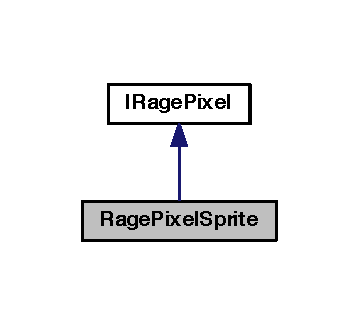
\includegraphics[width=172pt]{class_rage_pixel_sprite__inherit__graph}
\end{center}
\end{figure}


Collaboration diagram for Rage\-Pixel\-Sprite\-:
\nopagebreak
\begin{figure}[H]
\begin{center}
\leavevmode
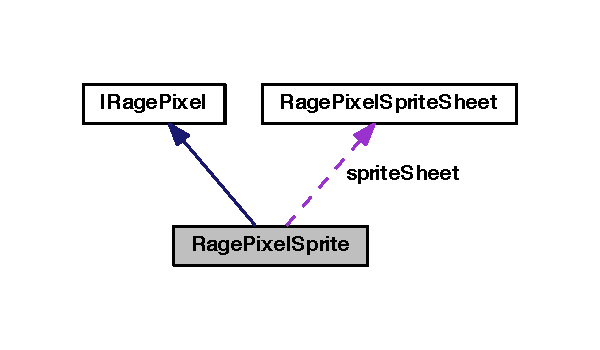
\includegraphics[width=288pt]{class_rage_pixel_sprite__coll__graph}
\end{center}
\end{figure}
\subsection*{Public Types}
\begin{DoxyCompactItemize}
\item 
enum {\bfseries Mode} 
\item 
enum {\bfseries Pivot\-Mode} 
\item 
enum {\bfseries Frame\-Mode} 
\item 
enum {\bfseries Animation\-Mode} 
\end{DoxyCompactItemize}
\subsection*{Public Member Functions}
\begin{DoxyCompactItemize}
\item 
\hypertarget{class_rage_pixel_sprite_aa60b5d24d5f6c0be7bade68db5f8b075}{void {\bfseries Snap\-To\-Scale} ()}\label{class_rage_pixel_sprite_aa60b5d24d5f6c0be7bade68db5f8b075}

\item 
\hypertarget{class_rage_pixel_sprite_ae1059c4949d908e5f172d75b6a0096c0}{void {\bfseries Snap\-To\-Integer\-Position} ()}\label{class_rage_pixel_sprite_ae1059c4949d908e5f172d75b6a0096c0}

\item 
\hypertarget{class_rage_pixel_sprite_ae84dba5aa3632b2f461b3753f788ebf6}{void {\bfseries Snap\-To\-Integer\-Position} (float divider)}\label{class_rage_pixel_sprite_ae84dba5aa3632b2f461b3753f788ebf6}

\item 
\hypertarget{class_rage_pixel_sprite_a54896121f8e0fbbd29ff1c781ca3dfb2}{void {\bfseries refresh\-Mesh} ()}\label{class_rage_pixel_sprite_a54896121f8e0fbbd29ff1c781ca3dfb2}

\item 
\hypertarget{class_rage_pixel_sprite_a69d82f22f591cc8a77ae931fa3d38e75}{void {\bfseries Generate\-Mesh} (Mesh mesh)}\label{class_rage_pixel_sprite_a69d82f22f591cc8a77ae931fa3d38e75}

\item 
\hypertarget{class_rage_pixel_sprite_a56213f3932debdd80ae56f4b7e856d0e}{void {\bfseries check\-Key\-Integrity} ()}\label{class_rage_pixel_sprite_a56213f3932debdd80ae56f4b7e856d0e}

\item 
\hypertarget{class_rage_pixel_sprite_ad4d681e3606ad2f4837e040982dd4605}{void {\bfseries On\-Destroy} ()}\label{class_rage_pixel_sprite_ad4d681e3606ad2f4837e040982dd4605}

\item 
\hypertarget{class_rage_pixel_sprite_a26f052fdd8c540b3f55332683961bdd1}{void {\bfseries shift\-Cell} (int amount, bool loop)}\label{class_rage_pixel_sprite_a26f052fdd8c540b3f55332683961bdd1}

\item 
\hypertarget{class_rage_pixel_sprite_a49eab8b050d780696d4d26d156434ffb}{void {\bfseries shift\-Row} (int amount)}\label{class_rage_pixel_sprite_a49eab8b050d780696d4d26d156434ffb}

\item 
\hypertarget{class_rage_pixel_sprite_aea82ffd60a3bb518abb7bb0f7b2bc69f}{void {\bfseries select\-Row} (int index)}\label{class_rage_pixel_sprite_aea82ffd60a3bb518abb7bb0f7b2bc69f}

\item 
\hypertarget{class_rage_pixel_sprite_a1962993215524923e1c810ad90cebd8b}{void {\bfseries select\-Cell} (int index)}\label{class_rage_pixel_sprite_a1962993215524923e1c810ad90cebd8b}

\item 
\hypertarget{class_rage_pixel_sprite_a2ccb4cc0dc2301d996308f40afc4dbbd}{string {\bfseries get\-Current\-Row\-Name} ()}\label{class_rage_pixel_sprite_a2ccb4cc0dc2301d996308f40afc4dbbd}

\item 
\hypertarget{class_rage_pixel_sprite_a5e71cfc0240f1efe2b4df41c2c098770}{\hyperlink{class_rage_pixel_row}{Rage\-Pixel\-Row} {\bfseries Get\-Current\-Row} ()}\label{class_rage_pixel_sprite_a5e71cfc0240f1efe2b4df41c2c098770}

\item 
\hypertarget{class_rage_pixel_sprite_a12a45416212f8a063b374ddffdaa4b16}{\hyperlink{class_rage_pixel_cell}{Rage\-Pixel\-Cell} {\bfseries Get\-Current\-Cell} ()}\label{class_rage_pixel_sprite_a12a45416212f8a063b374ddffdaa4b16}

\item 
\hypertarget{class_rage_pixel_sprite_af92a476b41f2377745fdf77276d51dd7}{int {\bfseries Get\-Current\-Cell\-Index} ()}\label{class_rage_pixel_sprite_af92a476b41f2377745fdf77276d51dd7}

\item 
\hypertarget{class_rage_pixel_sprite_a5a491eeabc7dddeff6e71fb89401a05e}{int {\bfseries Get\-Current\-Row\-Index} ()}\label{class_rage_pixel_sprite_a5a491eeabc7dddeff6e71fb89401a05e}

\item 
\hypertarget{class_rage_pixel_sprite_abd4ccc2ac4a713172d01954f09a79956}{void {\bfseries On\-Draw\-Gizmos\-Selected} ()}\label{class_rage_pixel_sprite_abd4ccc2ac4a713172d01954f09a79956}

\item 
\hypertarget{class_rage_pixel_sprite_a219cd468f9ed71ca548c104efcbd5a77}{void {\bfseries Set\-Sprite} (string name)}\label{class_rage_pixel_sprite_a219cd468f9ed71ca548c104efcbd5a77}

\item 
\hypertarget{class_rage_pixel_sprite_a1f6fd98f4d022d3e3bcec092a6b82edf}{void {\bfseries Set\-Sprite} (string name, int frame\-Index)}\label{class_rage_pixel_sprite_a1f6fd98f4d022d3e3bcec092a6b82edf}

\item 
\hypertarget{class_rage_pixel_sprite_ac506ca3a0d23206f0001e5cefd798863}{int {\bfseries Get\-Size\-X} ()}\label{class_rage_pixel_sprite_ac506ca3a0d23206f0001e5cefd798863}

\item 
\hypertarget{class_rage_pixel_sprite_a5a63873e353ef9291a5f265e4e3baff0}{int {\bfseries Get\-Size\-Y} ()}\label{class_rage_pixel_sprite_a5a63873e353ef9291a5f265e4e3baff0}

\item 
\hypertarget{class_rage_pixel_sprite_ae557b68f6e00fe1db13c875eaf02b1ac}{void {\bfseries Play\-Animation} ()}\label{class_rage_pixel_sprite_ae557b68f6e00fe1db13c875eaf02b1ac}

\item 
\hypertarget{class_rage_pixel_sprite_ad4ec1d4f93bbc698c67469baf5c3ec2e}{void {\bfseries Play\-Animation} (bool force\-Restart)}\label{class_rage_pixel_sprite_ad4ec1d4f93bbc698c67469baf5c3ec2e}

\item 
\hypertarget{class_rage_pixel_sprite_a5187d2f5a02e4a22b05cdc2f630f2f4c}{void {\bfseries Play\-Animation} (bool force\-Restart, int range\-Min\-Index, int range\-Max\-Index, int pri=0)}\label{class_rage_pixel_sprite_a5187d2f5a02e4a22b05cdc2f630f2f4c}

\item 
\hypertarget{class_rage_pixel_sprite_a2afe47975aca01efb29dcca92053baea}{void {\bfseries Play\-Animation} (bool force\-Restart, int\mbox{[}$\,$\mbox{]} frames, int pri=0)}\label{class_rage_pixel_sprite_a2afe47975aca01efb29dcca92053baea}

\item 
\hypertarget{class_rage_pixel_sprite_af8fdce57834b01a7b7b9f89a2c559455}{void {\bfseries Play\-Animation} (bool force\-Restart, Animation\-Mode anim\-Mode, int range\-Min\-Index, int range\-Max\-Index, int pri=0)}\label{class_rage_pixel_sprite_af8fdce57834b01a7b7b9f89a2c559455}

\item 
\hypertarget{class_rage_pixel_sprite_a72d3d3695e99a5c19703c17efe2d8b54}{void {\bfseries Play\-Animation} (bool force\-Restart, Animation\-Mode anim\-Mode, int\mbox{[}$\,$\mbox{]} frames, int pri=0)}\label{class_rage_pixel_sprite_a72d3d3695e99a5c19703c17efe2d8b54}

\item 
\hypertarget{class_rage_pixel_sprite_a870af117bb9a63e9e6b6c5c4587d84e3}{void {\bfseries Check\-Anim\-On\-Play} ()}\label{class_rage_pixel_sprite_a870af117bb9a63e9e6b6c5c4587d84e3}

\item 
\hypertarget{class_rage_pixel_sprite_a8099728fcb040eb0df549263f58a1a43}{bool {\bfseries Has\-Named\-Animation} (string name)}\label{class_rage_pixel_sprite_a8099728fcb040eb0df549263f58a1a43}

\item 
\hypertarget{class_rage_pixel_sprite_a8096c5255560cb25ee9af38282825bf2}{void {\bfseries Play\-Named\-Animation} (string name, int pri=0)}\label{class_rage_pixel_sprite_a8096c5255560cb25ee9af38282825bf2}

\item 
\hypertarget{class_rage_pixel_sprite_a55e3e799da237798826536b4c8e0358b}{void {\bfseries Play\-Named\-Animation} (string name, bool force\-Restart, int pri=0)}\label{class_rage_pixel_sprite_a55e3e799da237798826536b4c8e0358b}

\item 
\hypertarget{class_rage_pixel_sprite_a8d7023360b540e206c3a2c15e6f0801a}{bool {\bfseries Animation\-Is\-Different} (\hyperlink{class_rage_pixel_animation}{Rage\-Pixel\-Animation} a)}\label{class_rage_pixel_sprite_a8d7023360b540e206c3a2c15e6f0801a}

\item 
\hypertarget{class_rage_pixel_sprite_ab70e1719c79f8e0589e2bdb8c8c54bcf}{void {\bfseries Play\-Named\-Animation} (string name, bool force\-Restart, float delay\-First\-Frame, int pri=0)}\label{class_rage_pixel_sprite_ab70e1719c79f8e0589e2bdb8c8c54bcf}

\item 
\hypertarget{class_rage_pixel_sprite_a54be5b5042a4ba6823ba6aee7fdf45db}{void {\bfseries Stop\-Animation} ()}\label{class_rage_pixel_sprite_a54be5b5042a4ba6823ba6aee7fdf45db}

\item 
\hypertarget{class_rage_pixel_sprite_a7bb73e4f901a24ebd575741b039406cf}{bool {\bfseries is\-Playing} ()}\label{class_rage_pixel_sprite_a7bb73e4f901a24ebd575741b039406cf}

\item 
\hypertarget{class_rage_pixel_sprite_a839ac9cf6b178d5631b5b6dd8e5d81ab}{void {\bfseries Set\-Size} (int height, int width)}\label{class_rage_pixel_sprite_a839ac9cf6b178d5631b5b6dd8e5d81ab}

\item 
\hypertarget{class_rage_pixel_sprite_afd16f57c9ad6f99ff45a46fa518d6562}{Rect {\bfseries Get\-Rect} ()}\label{class_rage_pixel_sprite_afd16f57c9ad6f99ff45a46fa518d6562}

\item 
\hypertarget{class_rage_pixel_sprite_a9dfc4a8d48515b3e273c2f8488ac6559}{Vector3 {\bfseries Get\-Pivot\-Offset} ()}\label{class_rage_pixel_sprite_a9dfc4a8d48515b3e273c2f8488ac6559}

\item 
\hypertarget{class_rage_pixel_sprite_ae63857ebad450061821f45adb2989c03}{void {\bfseries Set\-Horizontal\-Flip} (bool value)}\label{class_rage_pixel_sprite_ae63857ebad450061821f45adb2989c03}

\item 
\hypertarget{class_rage_pixel_sprite_a633521badd38ad281a51d97a84c9e3bf}{void {\bfseries Set\-Vertical\-Flip} (bool value)}\label{class_rage_pixel_sprite_a633521badd38ad281a51d97a84c9e3bf}

\item 
\hypertarget{class_rage_pixel_sprite_a4d2cdda97935f9554088c3a3d2fd24fe}{void {\bfseries Set\-Tint\-Color} (Color color)}\label{class_rage_pixel_sprite_a4d2cdda97935f9554088c3a3d2fd24fe}

\end{DoxyCompactItemize}
\subsection*{Public Attributes}
\begin{DoxyCompactItemize}
\item 
\hypertarget{class_rage_pixel_sprite_ab1361e86e94e2b50037db46da41070c3}{Vector3 {\bfseries accurate\-Position}}\label{class_rage_pixel_sprite_ab1361e86e94e2b50037db46da41070c3}

\item 
\hypertarget{class_rage_pixel_sprite_a4b40d18f2b3f8d91f226a930d389198b}{\hyperlink{class_rage_pixel_sprite_sheet}{Rage\-Pixel\-Sprite\-Sheet} {\bfseries sprite\-Sheet}}\label{class_rage_pixel_sprite_a4b40d18f2b3f8d91f226a930d389198b}

\item 
\hypertarget{class_rage_pixel_sprite_a456f5c61113e978a23ee21ef4d0c1147}{Mode {\bfseries mode} = Mode.\-Default}\label{class_rage_pixel_sprite_a456f5c61113e978a23ee21ef4d0c1147}

\item 
\hypertarget{class_rage_pixel_sprite_a9512abd7d61b396deb721588352d8ee5}{Pivot\-Mode {\bfseries pivot\-Mode} = Pivot\-Mode.\-Bottom\-Left}\label{class_rage_pixel_sprite_a9512abd7d61b396deb721588352d8ee5}

\item 
\hypertarget{class_rage_pixel_sprite_a8ee328d09e16a05f248e534ce48f1b3f}{Frame\-Mode {\bfseries frame\-Mode} = 0}\label{class_rage_pixel_sprite_a8ee328d09e16a05f248e534ce48f1b3f}

\item 
\hypertarget{class_rage_pixel_sprite_a00714fbbb9420558f08fd509b6e4cca0}{Animation\-Mode {\bfseries animation\-Mode} = 0}\label{class_rage_pixel_sprite_a00714fbbb9420558f08fd509b6e4cca0}

\item 
\hypertarget{class_rage_pixel_sprite_ab096e6c7a8822c934326d8393021936c}{int {\bfseries animation\-Min\-Index} = -\/1}\label{class_rage_pixel_sprite_ab096e6c7a8822c934326d8393021936c}

\item 
\hypertarget{class_rage_pixel_sprite_a4497ca1de404d818ab6f3b7c9eb41534}{int {\bfseries animation\-Max\-Index} = -\/1}\label{class_rage_pixel_sprite_a4497ca1de404d818ab6f3b7c9eb41534}

\item 
\hypertarget{class_rage_pixel_sprite_a9da2483664103a922cd39edefbbf8b2a}{int\mbox{[}$\,$\mbox{]} {\bfseries animation\-Frames}}\label{class_rage_pixel_sprite_a9da2483664103a922cd39edefbbf8b2a}

\item 
\hypertarget{class_rage_pixel_sprite_aa9d8346e974a07784e1c2fd40b21d15a}{int {\bfseries animation\-Current\-Frame} = 0}\label{class_rage_pixel_sprite_aa9d8346e974a07784e1c2fd40b21d15a}

\item 
\hypertarget{class_rage_pixel_sprite_a74e273fa0b13c9e0e0280c4974b55e9f}{int {\bfseries grid9\-Left}}\label{class_rage_pixel_sprite_a74e273fa0b13c9e0e0280c4974b55e9f}

\item 
\hypertarget{class_rage_pixel_sprite_a39362b25073517762d8a89351d6518d3}{int {\bfseries grid9\-Top}}\label{class_rage_pixel_sprite_a39362b25073517762d8a89351d6518d3}

\item 
\hypertarget{class_rage_pixel_sprite_adcfc072011c4e5a1f6077f0336d8ffa4}{int {\bfseries grid9\-Right}}\label{class_rage_pixel_sprite_adcfc072011c4e5a1f6077f0336d8ffa4}

\item 
\hypertarget{class_rage_pixel_sprite_a61d9410920d499aca4f4478f5b8b303a}{int {\bfseries grid9\-Bottom}}\label{class_rage_pixel_sprite_a61d9410920d499aca4f4478f5b8b303a}

\item 
\hypertarget{class_rage_pixel_sprite_a845e21b1f2ef393cffd2ec007a0ee06a}{int {\bfseries current\-Row\-Key}}\label{class_rage_pixel_sprite_a845e21b1f2ef393cffd2ec007a0ee06a}

\item 
\hypertarget{class_rage_pixel_sprite_ab8448ec5efa4bf497f2eb1f89130a25c}{int {\bfseries current\-Cell\-Key}}\label{class_rage_pixel_sprite_ab8448ec5efa4bf497f2eb1f89130a25c}

\item 
\hypertarget{class_rage_pixel_sprite_a8e0975f63fe5ed896cf2d8d06a840452}{int {\bfseries Z\-Layer}}\label{class_rage_pixel_sprite_a8e0975f63fe5ed896cf2d8d06a840452}

\item 
\hypertarget{class_rage_pixel_sprite_a24f43766b5ad4ae05d199f58dc7345bc}{int {\bfseries pixel\-Size\-X} = 16}\label{class_rage_pixel_sprite_a24f43766b5ad4ae05d199f58dc7345bc}

\item 
\hypertarget{class_rage_pixel_sprite_a16da93a7a661108058fc653144832d4a}{int {\bfseries pixel\-Size\-Y} = 16}\label{class_rage_pixel_sprite_a16da93a7a661108058fc653144832d4a}

\item 
\hypertarget{class_rage_pixel_sprite_aa66cf5c516c4cecba047f7f9722a3239}{bool {\bfseries mesh\-Is\-Dirty} = false}\label{class_rage_pixel_sprite_aa66cf5c516c4cecba047f7f9722a3239}

\item 
\hypertarget{class_rage_pixel_sprite_a153fdf311739ac6f6f8a609147fe6496}{bool {\bfseries vertex\-Colors\-Are\-Dirty} = false}\label{class_rage_pixel_sprite_a153fdf311739ac6f6f8a609147fe6496}

\item 
\hypertarget{class_rage_pixel_sprite_a47dbafad6f1fe9f303e811edccf3ff5d}{Color {\bfseries tint\-Color} = new Color(1f, 1f, 1f, 1f)}\label{class_rage_pixel_sprite_a47dbafad6f1fe9f303e811edccf3ff5d}

\item 
\hypertarget{class_rage_pixel_sprite_af14cc6f8dcd319aad333cbdbb6b00c55}{bool {\bfseries flip\-Horizontal}}\label{class_rage_pixel_sprite_af14cc6f8dcd319aad333cbdbb6b00c55}

\item 
\hypertarget{class_rage_pixel_sprite_a2695b0925094cbef73d3aeff25f9245e}{bool {\bfseries flip\-Vertical}}\label{class_rage_pixel_sprite_a2695b0925094cbef73d3aeff25f9245e}

\item 
\hypertarget{class_rage_pixel_sprite_aec5016d6d460735781a2e2633739098e}{float {\bfseries next\-Anim\-Frame} = 0f}\label{class_rage_pixel_sprite_aec5016d6d460735781a2e2633739098e}

\item 
\hypertarget{class_rage_pixel_sprite_a58919b9ed71ac34a2a140d9b76f7b5d9}{bool {\bfseries play\-Animation} = false}\label{class_rage_pixel_sprite_a58919b9ed71ac34a2a140d9b76f7b5d9}

\end{DoxyCompactItemize}


\subsection{Detailed Description}


Definition at line 5 of file Rage\-Pixel\-Sprite.\-cs.



The documentation for this class was generated from the following file\-:\begin{DoxyCompactItemize}
\item 
assets/\-Rage\-Pixel/\-Rage\-Pixel\-Mono\-Develop/code/Rage\-Pixel\-Sprite.\-cs\end{DoxyCompactItemize}

\hypertarget{class_rage_pixel_sprite_editor}{\section{Rage\-Pixel\-Sprite\-Editor Class Reference}
\label{class_rage_pixel_sprite_editor}\index{Rage\-Pixel\-Sprite\-Editor@{Rage\-Pixel\-Sprite\-Editor}}
}
\subsection*{Public Types}
\begin{DoxyCompactItemize}
\item 
enum {\bfseries Mode} 
\item 
enum {\bfseries Brush\-Type} 
\end{DoxyCompactItemize}
\subsection*{Public Member Functions}
\begin{DoxyCompactItemize}
\item 
\hypertarget{class_rage_pixel_sprite_editor_a703dd66063d0f6c6a9d82d72b5ec1119}{void {\bfseries On\-Destroy} ()}\label{class_rage_pixel_sprite_editor_a703dd66063d0f6c6a9d82d72b5ec1119}

\item 
\hypertarget{class_rage_pixel_sprite_editor_a57674859bb00c2af0f92e7015fc0ad13}{override void {\bfseries On\-Inspector\-G\-U\-I} ()}\label{class_rage_pixel_sprite_editor_a57674859bb00c2af0f92e7015fc0ad13}

\item 
\hypertarget{class_rage_pixel_sprite_editor_a082cb275014bd9311fd08308ed928141}{void {\bfseries On\-Scene\-G\-U\-I} ()}\label{class_rage_pixel_sprite_editor_a082cb275014bd9311fd08308ed928141}

\item 
\hypertarget{class_rage_pixel_sprite_editor_a973ba2ff7fadbccbf006ba87830b963f}{void {\bfseries Handle\-Mode\-Default} ()}\label{class_rage_pixel_sprite_editor_a973ba2ff7fadbccbf006ba87830b963f}

\item 
\hypertarget{class_rage_pixel_sprite_editor_ad0feb0ca5388e3f4dd434516313dd5ad}{void {\bfseries Handle\-Mode\-Pen} ()}\label{class_rage_pixel_sprite_editor_ad0feb0ca5388e3f4dd434516313dd5ad}

\item 
\hypertarget{class_rage_pixel_sprite_editor_a521b2672d069b69d3a571995307416d8}{void {\bfseries Handle\-Mode\-Fill} ()}\label{class_rage_pixel_sprite_editor_a521b2672d069b69d3a571995307416d8}

\item 
\hypertarget{class_rage_pixel_sprite_editor_a8b3e425e2486c17a190f005e00280c24}{void {\bfseries Handle\-Mode\-Select} ()}\label{class_rage_pixel_sprite_editor_a8b3e425e2486c17a190f005e00280c24}

\item 
\hypertarget{class_rage_pixel_sprite_editor_a341fec8628bc0ac48804235be1a7fb4c}{void {\bfseries Handle\-Mode\-Resize} ()}\label{class_rage_pixel_sprite_editor_a341fec8628bc0ac48804235be1a7fb4c}

\item 
\hypertarget{class_rage_pixel_sprite_editor_a8b5503b262b6075857da931765827225}{void {\bfseries Scene\-G\-U\-I\-Init} ()}\label{class_rage_pixel_sprite_editor_a8b5503b262b6075857da931765827225}

\item 
\hypertarget{class_rage_pixel_sprite_editor_a152eff60ce878f587944ed3edf0fa35c}{void {\bfseries Handle\-Color\-Picker\-G\-U\-I} ()}\label{class_rage_pixel_sprite_editor_a152eff60ce878f587944ed3edf0fa35c}

\item 
\hypertarget{class_rage_pixel_sprite_editor_aa649a55f3459233211b08d20a8f3becf}{void {\bfseries Handle\-Paint\-G\-U\-I} ()}\label{class_rage_pixel_sprite_editor_aa649a55f3459233211b08d20a8f3becf}

\item 
\hypertarget{class_rage_pixel_sprite_editor_a4a498d9ae58790a8e74a71fa7f9edb30}{void {\bfseries Handle\-Palette\-G\-U\-I} ()}\label{class_rage_pixel_sprite_editor_a4a498d9ae58790a8e74a71fa7f9edb30}

\item 
\hypertarget{class_rage_pixel_sprite_editor_a1f45e447118a04d65184985d1fa131aa}{void {\bfseries Handle\-Animation\-G\-U\-I} ()}\label{class_rage_pixel_sprite_editor_a1f45e447118a04d65184985d1fa131aa}

\item 
\hypertarget{class_rage_pixel_sprite_editor_a229e952e89aa9b5f12a12ee5674959df}{void {\bfseries Handle\-Keyboard} ()}\label{class_rage_pixel_sprite_editor_a229e952e89aa9b5f12a12ee5674959df}

\item 
\hypertarget{class_rage_pixel_sprite_editor_a6f015ee37d0984ddb036163918ff0dee}{void {\bfseries Handle\-Camera\-Warnings} ()}\label{class_rage_pixel_sprite_editor_a6f015ee37d0984ddb036163918ff0dee}

\item 
\hypertarget{class_rage_pixel_sprite_editor_a8ab6e2d3cf94b4796dc3d7fbb6dfdab4}{void {\bfseries On\-Selected} ()}\label{class_rage_pixel_sprite_editor_a8ab6e2d3cf94b4796dc3d7fbb6dfdab4}

\item 
\hypertarget{class_rage_pixel_sprite_editor_a7d4ee008b005cb9b3568325edcd872b2}{void {\bfseries Initialize\-Empty\-Project} ()}\label{class_rage_pixel_sprite_editor_a7d4ee008b005cb9b3568325edcd872b2}

\item 
\hypertarget{class_rage_pixel_sprite_editor_ad8bb695c6fa75d819a89dcf6c524a030}{void {\bfseries Draw\-Gizmos} ()}\label{class_rage_pixel_sprite_editor_ad8bb695c6fa75d819a89dcf6c524a030}

\item 
\hypertarget{class_rage_pixel_sprite_editor_a02c9dfbdd9cdc1583e4edbb127e42100}{void {\bfseries Draw\-Grid9\-Gizmo} ()}\label{class_rage_pixel_sprite_editor_a02c9dfbdd9cdc1583e4edbb127e42100}

\item 
\hypertarget{class_rage_pixel_sprite_editor_a937c11252a482e51e647b64a71c01614}{void {\bfseries Draw\-Sprite\-Bounds\-Gizmo} ()}\label{class_rage_pixel_sprite_editor_a937c11252a482e51e647b64a71c01614}

\item 
\hypertarget{class_rage_pixel_sprite_editor_a4dfeacf83cb129326ef074521454ecfa}{void {\bfseries cancel\-Color\-Replacing} ()}\label{class_rage_pixel_sprite_editor_a4dfeacf83cb129326ef074521454ecfa}

\item 
\hypertarget{class_rage_pixel_sprite_editor_a3a71bf8341e51b17fd396d7c8a25fac7}{void {\bfseries Save\-Paint\-Undo} ()}\label{class_rage_pixel_sprite_editor_a3a71bf8341e51b17fd396d7c8a25fac7}

\item 
\hypertarget{class_rage_pixel_sprite_editor_ad4cb484e17cb477049427d13790c21bb}{void {\bfseries Do\-Paint\-Undo} ()}\label{class_rage_pixel_sprite_editor_ad4cb484e17cb477049427d13790c21bb}

\item 
\hypertarget{class_rage_pixel_sprite_editor_a3a544568283528ebba2d8325e9b343c0}{void {\bfseries Draw\-Selection\-Box} ()}\label{class_rage_pixel_sprite_editor_a3a544568283528ebba2d8325e9b343c0}

\item 
\hypertarget{class_rage_pixel_sprite_editor_a93e781f61798e4e66e95550acd3f17b9}{void {\bfseries Handle\-Inspector\-Spritesheet\-Remove} ()}\label{class_rage_pixel_sprite_editor_a93e781f61798e4e66e95550acd3f17b9}

\item 
\hypertarget{class_rage_pixel_sprite_editor_a85bf0f47bd9e6a6c7d7488c7046d8dc5}{void {\bfseries Refresh\-Preview\-Layer} ()}\label{class_rage_pixel_sprite_editor_a85bf0f47bd9e6a6c7d7488c7046d8dc5}

\item 
\hypertarget{class_rage_pixel_sprite_editor_a2669880346c608f99177088e63145ac2}{void {\bfseries Flood\-Fill} (Color old\-Color, Color color, Texture2\-D tex, int f\-X, int f\-Y, int min\-X, int min\-Y, int max\-X, int max\-Y)}\label{class_rage_pixel_sprite_editor_a2669880346c608f99177088e63145ac2}

\item 
\hypertarget{class_rage_pixel_sprite_editor_a0c5f3d9da26f922911d57bd3bdb86c14}{Color\mbox{[}$\,$\mbox{]} {\bfseries get\-Scaled\-Image} (Texture2\-D src, int width, int height, Color bg\-Color)}\label{class_rage_pixel_sprite_editor_a0c5f3d9da26f922911d57bd3bdb86c14}

\item 
\hypertarget{class_rage_pixel_sprite_editor_a5ba80f510b8538d1d7a49ef7dd2221a9}{void {\bfseries Show\-Debug\-Info} ()}\label{class_rage_pixel_sprite_editor_a5ba80f510b8538d1d7a49ef7dd2221a9}

\item 
\hypertarget{class_rage_pixel_sprite_editor_a817f7ee826ab5510a5c045a9361f4104}{\hyperlink{class_rage_pixel_texel}{Rage\-Pixel\-Texel} {\bfseries World\-To\-Texel\-Coords} (Texture2\-D tex, Transform t, Vector3 world\-Pos)}\label{class_rage_pixel_sprite_editor_a817f7ee826ab5510a5c045a9361f4104}

\item 
\hypertarget{class_rage_pixel_sprite_editor_a0532309139a8f9f7c4c5b6e71062c3d3}{Vector3 {\bfseries Get\-Pivot\-Offset} ()}\label{class_rage_pixel_sprite_editor_a0532309139a8f9f7c4c5b6e71062c3d3}

\item 
\hypertarget{class_rage_pixel_sprite_editor_ac8c634d551c16e7ca5c561b79e7bcfbf}{Vector3 {\bfseries Texel\-Coords\-To\-World} (Texture2\-D tex, Transform t, \hyperlink{class_rage_pixel_texel}{Rage\-Pixel\-Texel} texel)}\label{class_rage_pixel_sprite_editor_ac8c634d551c16e7ca5c561b79e7bcfbf}

\item 
\hypertarget{class_rage_pixel_sprite_editor_ac8178fe128b2c547d150dc9ee9644459}{Vector3 {\bfseries world\-To\-Scene\-Screen\-Point} (Vector3 world\-Pos)}\label{class_rage_pixel_sprite_editor_ac8178fe128b2c547d150dc9ee9644459}

\item 
\hypertarget{class_rage_pixel_sprite_editor_a2ed39c97d527f8d25909bdbaf99321e8}{Vector3 {\bfseries scene\-Screen\-To\-World\-Point} (Vector3 scene\-Screen\-Point)}\label{class_rage_pixel_sprite_editor_a2ed39c97d527f8d25909bdbaf99321e8}

\item 
\hypertarget{class_rage_pixel_sprite_editor_a95997ede63bd3c96b68026269dab5f66}{void {\bfseries save\-Texture} ()}\label{class_rage_pixel_sprite_editor_a95997ede63bd3c96b68026269dab5f66}

\item 
\hypertarget{class_rage_pixel_sprite_editor_a0be8ecb3a13b6b780a202be089ccd1f8}{\hyperlink{class_rage_pixel_bitmap}{Rage\-Pixel\-Bitmap} {\bfseries Grab\-Sprite} (Rect sprite\-U\-V)}\label{class_rage_pixel_sprite_editor_a0be8ecb3a13b6b780a202be089ccd1f8}

\item 
\hypertarget{class_rage_pixel_sprite_editor_a410c24a826310dff5a0a09a05064d96e}{\hyperlink{class_rage_pixel_bitmap}{Rage\-Pixel\-Bitmap} {\bfseries Grab\-Rect\-From\-Spritesheet} (\hyperlink{class_rage_pixel_texel_rect}{Rage\-Pixel\-Texel\-Rect} rect)}\label{class_rage_pixel_sprite_editor_a410c24a826310dff5a0a09a05064d96e}

\item 
\hypertarget{class_rage_pixel_sprite_editor_a12ca192ebb349ffaccc9d53f1805ef85}{void {\bfseries Cut\-Rect\-In\-Spritesheet} (\hyperlink{class_rage_pixel_texel_rect}{Rage\-Pixel\-Texel\-Rect} rect, Rect sprite\-U\-V)}\label{class_rage_pixel_sprite_editor_a12ca192ebb349ffaccc9d53f1805ef85}

\item 
\hypertarget{class_rage_pixel_sprite_editor_a2abd45da3cab0deeca35b1a35d536cde}{void {\bfseries Paste\-Bitmap\-To\-Spritesheet} (\hyperlink{class_rage_pixel_texel}{Rage\-Pixel\-Texel} position, Rect sprite\-U\-V, \hyperlink{class_rage_pixel_bitmap}{Rage\-Pixel\-Bitmap} bitmap)}\label{class_rage_pixel_sprite_editor_a2abd45da3cab0deeca35b1a35d536cde}

\item 
\hypertarget{class_rage_pixel_sprite_editor_af24a50a2a9395d577a2cf20581930e22}{void {\bfseries Paste\-Bitmap\-To\-Spritesheet\-Alpha} (\hyperlink{class_rage_pixel_texel}{Rage\-Pixel\-Texel} position, Rect sprite\-U\-V, \hyperlink{class_rage_pixel_bitmap}{Rage\-Pixel\-Bitmap} bitmap)}\label{class_rage_pixel_sprite_editor_af24a50a2a9395d577a2cf20581930e22}

\item 
\hypertarget{class_rage_pixel_sprite_editor_aa88987839d4c79686893913826ffc484}{void {\bfseries Invoke\-On\-Selected\-Event} ()}\label{class_rage_pixel_sprite_editor_aa88987839d4c79686893913826ffc484}

\item 
\hypertarget{class_rage_pixel_sprite_editor_add5dfd38c1894275f4f6a3b75d6e2f0b}{Camera {\bfseries Get\-Scene\-Camera} ()}\label{class_rage_pixel_sprite_editor_add5dfd38c1894275f4f6a3b75d6e2f0b}

\item 
\hypertarget{class_rage_pixel_sprite_editor_a45f096459edb8fd0118ce4a9750cf83f}{int {\bfseries Get\-Atlas\-Cell\-Count} (\hyperlink{class_rage_pixel_sprite_sheet}{Rage\-Pixel\-Sprite\-Sheet}\mbox{[}$\,$\mbox{]} sprite\-Sheets, Material atlas)}\label{class_rage_pixel_sprite_editor_a45f096459edb8fd0118ce4a9750cf83f}

\item 
\hypertarget{class_rage_pixel_sprite_editor_ac1fda321f7e80ea33ce3aa1f37cb1f0b}{bool {\bfseries Scene\-Camera\-Facing\-Correctly} ()}\label{class_rage_pixel_sprite_editor_ac1fda321f7e80ea33ce3aa1f37cb1f0b}

\item 
\hypertarget{class_rage_pixel_sprite_editor_a0d8e7bcb9d8066536c93dc6b347008b5}{Color {\bfseries Get\-Scene\-Button\-Color} (bool active)}\label{class_rage_pixel_sprite_editor_a0d8e7bcb9d8066536c93dc6b347008b5}

\end{DoxyCompactItemize}
\subsection*{Public Attributes}
\begin{DoxyCompactItemize}
\item 
\hypertarget{class_rage_pixel_sprite_editor_aa22fd81df35bcf7e4a2b2fe06d21bc64}{Mode {\bfseries mode} = Mode.\-Default}\label{class_rage_pixel_sprite_editor_aa22fd81df35bcf7e4a2b2fe06d21bc64}

\item 
\hypertarget{class_rage_pixel_sprite_editor_ad35b0f96df30dfcf4e0e15ca920485b4}{Vector2 {\bfseries rectangle\-Start}}\label{class_rage_pixel_sprite_editor_ad35b0f96df30dfcf4e0e15ca920485b4}

\item 
\hypertarget{class_rage_pixel_sprite_editor_a985891f307eeeaf65c9941d33908b26a}{Brush\-Type {\bfseries brush\-Type} = Brush\-Type.\-Brush1}\label{class_rage_pixel_sprite_editor_a985891f307eeeaf65c9941d33908b26a}

\end{DoxyCompactItemize}
\subsection*{Protected Attributes}
\begin{DoxyCompactItemize}
\item 
\hypertarget{class_rage_pixel_sprite_editor_adc9ca5b140961362a8d950ff4016a65f}{bool {\bfseries animation\-Strip\-Enabled} = true}\label{class_rage_pixel_sprite_editor_adc9ca5b140961362a8d950ff4016a65f}

\end{DoxyCompactItemize}
\subsection*{Properties}
\begin{DoxyCompactItemize}
\item 
\hypertarget{class_rage_pixel_sprite_editor_a6f123c1c34b4a21495167dc415250bb1}{\hyperlink{class_rage_pixel_bitmap}{Rage\-Pixel\-Bitmap} {\bfseries brush}\hspace{0.3cm}{\ttfamily  \mbox{[}get\mbox{]}}}\label{class_rage_pixel_sprite_editor_a6f123c1c34b4a21495167dc415250bb1}

\item 
\hypertarget{class_rage_pixel_sprite_editor_a1f9778108172bd7641db90fc7e20c347}{Mesh\-Renderer {\bfseries mesh\-Renderer}\hspace{0.3cm}{\ttfamily  \mbox{[}get\mbox{]}}}\label{class_rage_pixel_sprite_editor_a1f9778108172bd7641db90fc7e20c347}

\item 
\hypertarget{class_rage_pixel_sprite_editor_a1f23f91644708d626bb089bd0cd56ba7}{Mesh\-Filter {\bfseries mesh\-Filter}\hspace{0.3cm}{\ttfamily  \mbox{[}get\mbox{]}}}\label{class_rage_pixel_sprite_editor_a1f23f91644708d626bb089bd0cd56ba7}

\item 
\hypertarget{class_rage_pixel_sprite_editor_aca2fbb26a33386e6e7ef07b2f6dd21aa}{Texture2\-D {\bfseries spritesheet\-Texture}\hspace{0.3cm}{\ttfamily  \mbox{[}get\mbox{]}}}\label{class_rage_pixel_sprite_editor_aca2fbb26a33386e6e7ef07b2f6dd21aa}

\item 
\hypertarget{class_rage_pixel_sprite_editor_a53fdfd957adbeafc33ed0efd7d252595}{\hyperlink{class_rage_pixel_sprite}{Rage\-Pixel\-Sprite} {\bfseries rage\-Pixel\-Sprite}\hspace{0.3cm}{\ttfamily  \mbox{[}get\mbox{]}}}\label{class_rage_pixel_sprite_editor_a53fdfd957adbeafc33ed0efd7d252595}

\item 
\hypertarget{class_rage_pixel_sprite_editor_ad36c2076eec016e664f2704d6994d14f}{\hyperlink{class_rage_pixel_anim_strip_g_u_i}{Rage\-Pixel\-Anim\-Strip\-G\-U\-I} {\bfseries anim\-Strip\-G\-U\-I}\hspace{0.3cm}{\ttfamily  \mbox{[}get\mbox{]}}}\label{class_rage_pixel_sprite_editor_ad36c2076eec016e664f2704d6994d14f}

\item 
\hypertarget{class_rage_pixel_sprite_editor_afe0768b737d8ea57833ec078c094e628}{\hyperlink{class_rage_pixel_sprite_sheet_g_u_i}{Rage\-Pixel\-Sprite\-Sheet\-G\-U\-I} {\bfseries sprite\-Sheet\-G\-U\-I}\hspace{0.3cm}{\ttfamily  \mbox{[}get\mbox{]}}}\label{class_rage_pixel_sprite_editor_afe0768b737d8ea57833ec078c094e628}

\item 
\hypertarget{class_rage_pixel_sprite_editor_a77d755c98139a5778aa663370f0f379b}{\hyperlink{class_rage_pixel_color_picker_g_u_i}{Rage\-Pixel\-Color\-Picker\-G\-U\-I} {\bfseries paint\-Color\-Picker\-G\-U\-I}\hspace{0.3cm}{\ttfamily  \mbox{[}get\mbox{]}}}\label{class_rage_pixel_sprite_editor_a77d755c98139a5778aa663370f0f379b}

\item 
\hypertarget{class_rage_pixel_sprite_editor_a8e27152ebda2379cad1f19a1a4017fbf}{\hyperlink{class_rage_pixel_color_picker_g_u_i}{Rage\-Pixel\-Color\-Picker\-G\-U\-I} {\bfseries replace\-Color\-Picker\-G\-U\-I}\hspace{0.3cm}{\ttfamily  \mbox{[}get\mbox{]}}}\label{class_rage_pixel_sprite_editor_a8e27152ebda2379cad1f19a1a4017fbf}

\end{DoxyCompactItemize}


\subsection{Detailed Description}


Definition at line 9 of file Rage\-Pixel\-Sprite\-Editor.\-cs.



The documentation for this class was generated from the following file\-:\begin{DoxyCompactItemize}
\item 
assets/\-Rage\-Pixel/\-Rage\-Pixel\-Mono\-Develop/editor/Rage\-Pixel\-Sprite\-Editor.\-cs\end{DoxyCompactItemize}

\hypertarget{class_rage_pixel_sprite_sheet}{\section{Rage\-Pixel\-Sprite\-Sheet Class Reference}
\label{class_rage_pixel_sprite_sheet}\index{Rage\-Pixel\-Sprite\-Sheet@{Rage\-Pixel\-Sprite\-Sheet}}
}
\subsection*{Public Member Functions}
\begin{DoxyCompactItemize}
\item 
\hypertarget{class_rage_pixel_sprite_sheet_a3085b28d0e238317cfcf7b9624f4b8ee}{\hyperlink{class_rage_pixel_row}{Rage\-Pixel\-Row} {\bfseries Add\-Row} (int key, int pixel\-Size\-X, int pixel\-Size\-Y)}\label{class_rage_pixel_sprite_sheet_a3085b28d0e238317cfcf7b9624f4b8ee}

\item 
\hypertarget{class_rage_pixel_sprite_sheet_a4f9d8ec6a99d9ae31d5974efd554039d}{\hyperlink{class_rage_pixel_row}{Rage\-Pixel\-Row} {\bfseries Add\-Row} (int key, int index, int pixel\-Size\-X, int pixel\-Size\-Y)}\label{class_rage_pixel_sprite_sheet_a4f9d8ec6a99d9ae31d5974efd554039d}

\item 
\hypertarget{class_rage_pixel_sprite_sheet_aa241db4f20308246c2b70b059304755b}{void {\bfseries Move\-Row} (int from\-Index, int to\-Index)}\label{class_rage_pixel_sprite_sheet_aa241db4f20308246c2b70b059304755b}

\item 
\hypertarget{class_rage_pixel_sprite_sheet_ab54e8274c3cd2a256b7b2befb680c3e4}{\hyperlink{class_rage_pixel_row}{Rage\-Pixel\-Row} {\bfseries Get\-Row} (int key)}\label{class_rage_pixel_sprite_sheet_ab54e8274c3cd2a256b7b2befb680c3e4}

\item 
\hypertarget{class_rage_pixel_sprite_sheet_a500e37a0b7ba3f833f0f0c2c3207b3af}{\hyperlink{class_rage_pixel_row}{Rage\-Pixel\-Row} {\bfseries Get\-Row\-By\-Name} (string name)}\label{class_rage_pixel_sprite_sheet_a500e37a0b7ba3f833f0f0c2c3207b3af}

\item 
\hypertarget{class_rage_pixel_sprite_sheet_a71e69ac7a2154b8a7808c157f1ae1f32}{int {\bfseries Get\-Key} (int index)}\label{class_rage_pixel_sprite_sheet_a71e69ac7a2154b8a7808c157f1ae1f32}

\item 
\hypertarget{class_rage_pixel_sprite_sheet_aaf3851d67ec35485d84cbd940b2c04df}{int {\bfseries Get\-Index} (int key)}\label{class_rage_pixel_sprite_sheet_aaf3851d67ec35485d84cbd940b2c04df}

\item 
\hypertarget{class_rage_pixel_sprite_sheet_a11300c3042982073e0a597262f821ca5}{int {\bfseries Get\-Index\-By\-Name} (string name)}\label{class_rage_pixel_sprite_sheet_a11300c3042982073e0a597262f821ca5}

\item 
\hypertarget{class_rage_pixel_sprite_sheet_a14e0f896028db7cd3ba5f9b91296d9e2}{void {\bfseries Remove\-Row\-By\-Key} (int key)}\label{class_rage_pixel_sprite_sheet_a14e0f896028db7cd3ba5f9b91296d9e2}

\item 
\hypertarget{class_rage_pixel_sprite_sheet_a6c9d468880df0f7a32bee1b68706472a}{void {\bfseries Remove\-Row\-By\-Name} (string name)}\label{class_rage_pixel_sprite_sheet_a6c9d468880df0f7a32bee1b68706472a}

\item 
\hypertarget{class_rage_pixel_sprite_sheet_a8c731ec816c2851f8fbd3ca4a8e7be9f}{void {\bfseries Remove\-Row\-By\-Index} (int index)}\label{class_rage_pixel_sprite_sheet_a8c731ec816c2851f8fbd3ca4a8e7be9f}

\item 
\hypertarget{class_rage_pixel_sprite_sheet_afb25696fccd110b409bb90c2cfbeb4a0}{int {\bfseries Get\-Total\-Cell\-Count} ()}\label{class_rage_pixel_sprite_sheet_afb25696fccd110b409bb90c2cfbeb4a0}

\item 
\hypertarget{class_rage_pixel_sprite_sheet_a93454e8ef7e23d61acf7a988040de8bc}{void {\bfseries save\-Undo} (Color32\mbox{[}$\,$\mbox{]} buffer, \hyperlink{class_rage_pixel_cell}{Rage\-Pixel\-Cell} cell)}\label{class_rage_pixel_sprite_sheet_a93454e8ef7e23d61acf7a988040de8bc}

\item 
\hypertarget{class_rage_pixel_sprite_sheet_adf108aa4645abf42b61b0e04705b9ff1}{void {\bfseries save\-Undo} (\hyperlink{class_rage_pixel_cell}{Rage\-Pixel\-Cell} cell)}\label{class_rage_pixel_sprite_sheet_adf108aa4645abf42b61b0e04705b9ff1}

\item 
\hypertarget{class_rage_pixel_sprite_sheet_ae762040f2d1a0974f01479874c16dcf4}{void {\bfseries Do\-Undo} (\hyperlink{class_rage_pixel_cell}{Rage\-Pixel\-Cell} cell)}\label{class_rage_pixel_sprite_sheet_ae762040f2d1a0974f01479874c16dcf4}

\item 
\hypertarget{class_rage_pixel_sprite_sheet_a92c49828ae825af2ed039a5169308159}{Color {\bfseries replace\-Color} (Color32\mbox{[}$\,$\mbox{]} before, Color old\-Color, Color new\-Color)}\label{class_rage_pixel_sprite_sheet_a92c49828ae825af2ed039a5169308159}

\item 
\hypertarget{class_rage_pixel_sprite_sheet_aecfb7ff55fee7915eed484d07fd4beee}{Color {\bfseries replace\-Color} (Color32\mbox{[}$\,$\mbox{]} before, Color old\-Color, Color new\-Color, \hyperlink{class_rage_pixel_row}{Rage\-Pixel\-Row} target\-Row)}\label{class_rage_pixel_sprite_sheet_aecfb7ff55fee7915eed484d07fd4beee}

\item 
\hypertarget{class_rage_pixel_sprite_sheet_a1b3c548164ced39b6ccb469f58be9f46}{Color\mbox{[}$\,$\mbox{]} {\bfseries get\-Preview\-Image} (int row\-Index, int cell\-Index, int width, int height, bool selected, Color selected\-Border)}\label{class_rage_pixel_sprite_sheet_a1b3c548164ced39b6ccb469f58be9f46}

\item 
\hypertarget{class_rage_pixel_sprite_sheet_aee9d6159447f59b0ac1aa8608507cbf2}{Color\mbox{[}$\,$\mbox{]} {\bfseries get\-Image} (int row\-Index, int cell\-Index)}\label{class_rage_pixel_sprite_sheet_aee9d6159447f59b0ac1aa8608507cbf2}

\item 
\hypertarget{class_rage_pixel_sprite_sheet_ae2f0ce120f4f5489b631254c1b4fe1c0}{Color\mbox{[}$\,$\mbox{]} {\bfseries get\-Image} (int row\-Index, int cell\-Index, int left, int top, int width, int height)}\label{class_rage_pixel_sprite_sheet_ae2f0ce120f4f5489b631254c1b4fe1c0}

\end{DoxyCompactItemize}
\subsection*{Public Attributes}
\begin{DoxyCompactItemize}
\item 
\hypertarget{class_rage_pixel_sprite_sheet_a802f55e0ff17565a85c4407c33c0099b}{Material {\bfseries atlas}}\label{class_rage_pixel_sprite_sheet_a802f55e0ff17565a85c4407c33c0099b}

\item 
\hypertarget{class_rage_pixel_sprite_sheet_a1888bb9e536725e355e468b134683e30}{int {\bfseries thumbnail\-Size} = 40}\label{class_rage_pixel_sprite_sheet_a1888bb9e536725e355e468b134683e30}

\end{DoxyCompactItemize}
\subsection*{Properties}
\begin{DoxyCompactItemize}
\item 
\hypertarget{class_rage_pixel_sprite_sheet_a3f5b1ca6150b8aa47a899cc36c1fd8da}{\hyperlink{class_rage_pixel_row}{Rage\-Pixel\-Row}\mbox{[}$\,$\mbox{]} {\bfseries rows}\hspace{0.3cm}{\ttfamily  \mbox{[}get, set\mbox{]}}}\label{class_rage_pixel_sprite_sheet_a3f5b1ca6150b8aa47a899cc36c1fd8da}

\end{DoxyCompactItemize}


\subsection{Detailed Description}


Definition at line 5 of file Rage\-Pixel\-Sprite\-Sheet.\-cs.



The documentation for this class was generated from the following file\-:\begin{DoxyCompactItemize}
\item 
assets/\-Rage\-Pixel/\-Rage\-Pixel\-Mono\-Develop/code/Rage\-Pixel\-Sprite\-Sheet.\-cs\end{DoxyCompactItemize}

\hypertarget{class_rage_pixel_sprite_sheet_editor_window}{\section{Rage\-Pixel\-Sprite\-Sheet\-Editor\-Window Class Reference}
\label{class_rage_pixel_sprite_sheet_editor_window}\index{Rage\-Pixel\-Sprite\-Sheet\-Editor\-Window@{Rage\-Pixel\-Sprite\-Sheet\-Editor\-Window}}
}


Collaboration diagram for Rage\-Pixel\-Sprite\-Sheet\-Editor\-Window\-:
\nopagebreak
\begin{figure}[H]
\begin{center}
\leavevmode
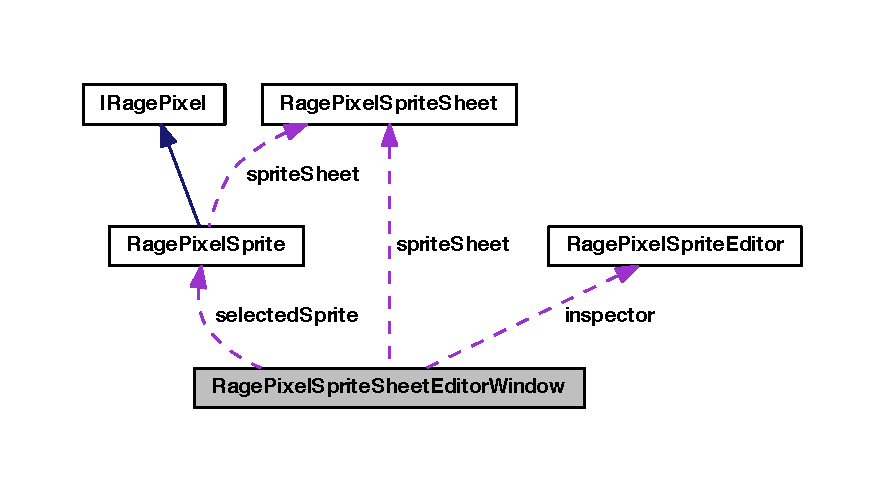
\includegraphics[width=350pt]{class_rage_pixel_sprite_sheet_editor_window__coll__graph}
\end{center}
\end{figure}
\subsection*{Public Types}
\begin{DoxyCompactItemize}
\item 
enum {\bfseries Sprite\-Sheet\-Import\-Target} 
\item 
enum {\bfseries Sprite\-Sheet\-Update\-Target} 
\end{DoxyCompactItemize}
\subsection*{Public Member Functions}
\begin{DoxyCompactItemize}
\item 
\hypertarget{class_rage_pixel_sprite_sheet_editor_window_ad2abff1de5b689d7c8ecabd64213b6d3}{void {\bfseries On\-G\-U\-I} ()}\label{class_rage_pixel_sprite_sheet_editor_window_ad2abff1de5b689d7c8ecabd64213b6d3}

\item 
\hypertarget{class_rage_pixel_sprite_sheet_editor_window_a2fdd9ac901809971b1f79437f8885416}{void {\bfseries Update} ()}\label{class_rage_pixel_sprite_sheet_editor_window_a2fdd9ac901809971b1f79437f8885416}

\item 
\hypertarget{class_rage_pixel_sprite_sheet_editor_window_ac6dabc031e6e6f37baa1a139582fad6f}{void {\bfseries On\-Destroy} ()}\label{class_rage_pixel_sprite_sheet_editor_window_ac6dabc031e6e6f37baa1a139582fad6f}

\item 
\hypertarget{class_rage_pixel_sprite_sheet_editor_window_ae6b2d647a8b0feb795a3966a7fb5b68e}{void {\bfseries Update\-Sprite} (Sprite\-Sheet\-Update\-Target target)}\label{class_rage_pixel_sprite_sheet_editor_window_ae6b2d647a8b0feb795a3966a7fb5b68e}

\item 
\hypertarget{class_rage_pixel_sprite_sheet_editor_window_a1de880bc4c4ab2722809f1e867dbdff8}{void {\bfseries Update\-Cell} (\hyperlink{class_rage_pixel_cell}{Rage\-Pixel\-Cell} cell, Texture2\-D spritesheet\-Texture)}\label{class_rage_pixel_sprite_sheet_editor_window_a1de880bc4c4ab2722809f1e867dbdff8}

\item 
\hypertarget{class_rage_pixel_sprite_sheet_editor_window_a25fb2b1e2876b3ab91389850027ed4cd}{void {\bfseries Import\-Sprite} (Sprite\-Sheet\-Import\-Target target)}\label{class_rage_pixel_sprite_sheet_editor_window_a25fb2b1e2876b3ab91389850027ed4cd}

\end{DoxyCompactItemize}
\subsection*{Public Attributes}
\begin{DoxyCompactItemize}
\item 
\hypertarget{class_rage_pixel_sprite_sheet_editor_window_a86ff0367c7f404395218fcee71124f42}{\hyperlink{class_rage_pixel_sprite_sheet}{Rage\-Pixel\-Sprite\-Sheet} {\bfseries sprite\-Sheet}}\label{class_rage_pixel_sprite_sheet_editor_window_a86ff0367c7f404395218fcee71124f42}

\item 
\hypertarget{class_rage_pixel_sprite_sheet_editor_window_a22e08ebd95ce65317e5e302486ebef3d}{\hyperlink{class_rage_pixel_sprite_editor}{Rage\-Pixel\-Sprite\-Editor} {\bfseries inspector}}\label{class_rage_pixel_sprite_sheet_editor_window_a22e08ebd95ce65317e5e302486ebef3d}

\item 
\hypertarget{class_rage_pixel_sprite_sheet_editor_window_ae55f59a21aec80b97d91122baa39d5b6}{\hyperlink{class_rage_pixel_sprite}{Rage\-Pixel\-Sprite} {\bfseries selected\-Sprite}}\label{class_rage_pixel_sprite_sheet_editor_window_ae55f59a21aec80b97d91122baa39d5b6}

\end{DoxyCompactItemize}
\subsection*{Properties}
\begin{DoxyCompactItemize}
\item 
\hypertarget{class_rage_pixel_sprite_sheet_editor_window_aa6509346df3bb405df0b4a62a5560595}{\hyperlink{class_rage_pixel_anim_strip_g_u_i}{Rage\-Pixel\-Anim\-Strip\-G\-U\-I} {\bfseries anim\-Strip\-G\-U\-I}\hspace{0.3cm}{\ttfamily  \mbox{[}get\mbox{]}}}\label{class_rage_pixel_sprite_sheet_editor_window_aa6509346df3bb405df0b4a62a5560595}

\item 
\hypertarget{class_rage_pixel_sprite_sheet_editor_window_a17abd4fc52a987957efd2b3593b6d160}{\hyperlink{class_rage_pixel_sprite_sheet_g_u_i}{Rage\-Pixel\-Sprite\-Sheet\-G\-U\-I} {\bfseries sprite\-Sheet\-G\-U\-I}\hspace{0.3cm}{\ttfamily  \mbox{[}get\mbox{]}}}\label{class_rage_pixel_sprite_sheet_editor_window_a17abd4fc52a987957efd2b3593b6d160}

\item 
\hypertarget{class_rage_pixel_sprite_sheet_editor_window_a219779fe46c4db7dbae9e4dcafede74f}{\hyperlink{class_rage_pixel_sprite_sheet_g_u_i}{Rage\-Pixel\-Sprite\-Sheet\-G\-U\-I} {\bfseries copy\-Sprite\-Sheet\-G\-U\-I}\hspace{0.3cm}{\ttfamily  \mbox{[}get\mbox{]}}}\label{class_rage_pixel_sprite_sheet_editor_window_a219779fe46c4db7dbae9e4dcafede74f}

\end{DoxyCompactItemize}


\subsection{Detailed Description}


Definition at line 6 of file Rage\-Pixel\-Sprite\-Sheet\-Editor\-Window.\-cs.



The documentation for this class was generated from the following file\-:\begin{DoxyCompactItemize}
\item 
assets/\-Rage\-Pixel/\-Rage\-Pixel\-Mono\-Develop/editor/Rage\-Pixel\-Sprite\-Sheet\-Editor\-Window.\-cs\end{DoxyCompactItemize}

\hypertarget{class_rage_pixel_sprite_sheet_g_u_i}{\section{Rage\-Pixel\-Sprite\-Sheet\-G\-U\-I Class Reference}
\label{class_rage_pixel_sprite_sheet_g_u_i}\index{Rage\-Pixel\-Sprite\-Sheet\-G\-U\-I@{Rage\-Pixel\-Sprite\-Sheet\-G\-U\-I}}
}
\subsection*{Public Member Functions}
\begin{DoxyCompactItemize}
\item 
\hypertarget{class_rage_pixel_sprite_sheet_g_u_i_a4bada9440adbd3700c363d29506773b5}{bool {\bfseries size\-Is\-Dirty} (int width)}\label{class_rage_pixel_sprite_sheet_g_u_i_a4bada9440adbd3700c363d29506773b5}

\item 
\hypertarget{class_rage_pixel_sprite_sheet_g_u_i_a52024c4d21cdaab9df2a9b6a4481712d}{void {\bfseries Create\-Texture\-Instance} ()}\label{class_rage_pixel_sprite_sheet_g_u_i_a52024c4d21cdaab9df2a9b6a4481712d}

\item 
\hypertarget{class_rage_pixel_sprite_sheet_g_u_i_ab9b95d2818a676750bf3c4b4a3744c20}{void {\bfseries Refresh} ()}\label{class_rage_pixel_sprite_sheet_g_u_i_ab9b95d2818a676750bf3c4b4a3744c20}

\item 
\hypertarget{class_rage_pixel_sprite_sheet_g_u_i_abb80ff910b04223d9cc746147218d791}{int {\bfseries Get\-Row\-Index} (int local\-X, int local\-Y)}\label{class_rage_pixel_sprite_sheet_g_u_i_abb80ff910b04223d9cc746147218d791}

\item 
\hypertarget{class_rage_pixel_sprite_sheet_g_u_i_a7be13e1e873d750f201124b74aace1af}{bool {\bfseries Handle\-G\-U\-I\-Event} (Event ev)}\label{class_rage_pixel_sprite_sheet_g_u_i_a7be13e1e873d750f201124b74aace1af}

\item 
\hypertarget{class_rage_pixel_sprite_sheet_g_u_i_aecfb82941eebcc8c8647463851acdf8c}{void {\bfseries Clean\-Exit} ()}\label{class_rage_pixel_sprite_sheet_g_u_i_aecfb82941eebcc8c8647463851acdf8c}

\end{DoxyCompactItemize}
\subsection*{Public Attributes}
\begin{DoxyCompactItemize}
\item 
Color {\bfseries background\-Color}
\item 
\hypertarget{class_rage_pixel_sprite_sheet_g_u_i_a62075f7ec1f088a38733772ee052028d}{bool {\bfseries anim\-Strip\-Is\-Dirty} = false}\label{class_rage_pixel_sprite_sheet_g_u_i_a62075f7ec1f088a38733772ee052028d}

\item 
\hypertarget{class_rage_pixel_sprite_sheet_g_u_i_a79c8fd88e1a12fc8a8152736bd9999ce}{bool {\bfseries is\-Dirty} = false}\label{class_rage_pixel_sprite_sheet_g_u_i_a79c8fd88e1a12fc8a8152736bd9999ce}

\item 
\hypertarget{class_rage_pixel_sprite_sheet_g_u_i_a38a5575ae6227847e80b3f6e07a3f6f7}{int {\bfseries drag\-Target\-Index} = -\/1}\label{class_rage_pixel_sprite_sheet_g_u_i_a38a5575ae6227847e80b3f6e07a3f6f7}

\item 
\hypertarget{class_rage_pixel_sprite_sheet_g_u_i_a23d671c82962ed666bc6450f907c7ef7}{int {\bfseries position\-X}}\label{class_rage_pixel_sprite_sheet_g_u_i_a23d671c82962ed666bc6450f907c7ef7}

\item 
\hypertarget{class_rage_pixel_sprite_sheet_g_u_i_a66aca83246ddf0cb69e7f2b27f3af1fa}{int {\bfseries position\-Y}}\label{class_rage_pixel_sprite_sheet_g_u_i_a66aca83246ddf0cb69e7f2b27f3af1fa}

\end{DoxyCompactItemize}
\subsection*{Properties}
\begin{DoxyCompactItemize}
\item 
\hypertarget{class_rage_pixel_sprite_sheet_g_u_i_abc17e862d34b73e9c62859cfc9d12a59}{Rect {\bfseries bounds}\hspace{0.3cm}{\ttfamily  \mbox{[}get\mbox{]}}}\label{class_rage_pixel_sprite_sheet_g_u_i_abc17e862d34b73e9c62859cfc9d12a59}

\item 
\hypertarget{class_rage_pixel_sprite_sheet_g_u_i_a092e41dce55b46f61c8c10d5c9006194}{\hyperlink{class_rage_pixel_sprite_sheet}{Rage\-Pixel\-Sprite\-Sheet} {\bfseries sprite\-Sheet}\hspace{0.3cm}{\ttfamily  \mbox{[}get, set\mbox{]}}}\label{class_rage_pixel_sprite_sheet_g_u_i_a092e41dce55b46f61c8c10d5c9006194}

\item 
\hypertarget{class_rage_pixel_sprite_sheet_g_u_i_a4c3065bda9f32f5ce3b41f547ba8ffba}{int {\bfseries max\-Width}\hspace{0.3cm}{\ttfamily  \mbox{[}get, set\mbox{]}}}\label{class_rage_pixel_sprite_sheet_g_u_i_a4c3065bda9f32f5ce3b41f547ba8ffba}

\item 
\hypertarget{class_rage_pixel_sprite_sheet_g_u_i_a2a5e4e0ae3fc5791489b5b88633bb688}{Texture2\-D {\bfseries sprite\-Sheet\-Texture}\hspace{0.3cm}{\ttfamily  \mbox{[}get\mbox{]}}}\label{class_rage_pixel_sprite_sheet_g_u_i_a2a5e4e0ae3fc5791489b5b88633bb688}

\item 
\hypertarget{class_rage_pixel_sprite_sheet_g_u_i_a1f64b6e6f552045d97590ea0311ff2fb}{int {\bfseries current\-Row\-Key}\hspace{0.3cm}{\ttfamily  \mbox{[}get, set\mbox{]}}}\label{class_rage_pixel_sprite_sheet_g_u_i_a1f64b6e6f552045d97590ea0311ff2fb}

\item 
\hypertarget{class_rage_pixel_sprite_sheet_g_u_i_a114bb335d2e46e65b776279ec2c6dd68}{int {\bfseries table\-Width}\hspace{0.3cm}{\ttfamily  \mbox{[}get\mbox{]}}}\label{class_rage_pixel_sprite_sheet_g_u_i_a114bb335d2e46e65b776279ec2c6dd68}

\item 
\hypertarget{class_rage_pixel_sprite_sheet_g_u_i_a9dde0a87194dac22f9ed51656533ad8c}{int {\bfseries table\-Height}\hspace{0.3cm}{\ttfamily  \mbox{[}get\mbox{]}}}\label{class_rage_pixel_sprite_sheet_g_u_i_a9dde0a87194dac22f9ed51656533ad8c}

\item 
\hypertarget{class_rage_pixel_sprite_sheet_g_u_i_a68722f6143d204cb847f5ebfe5b9d300}{int {\bfseries pixel\-Width}\hspace{0.3cm}{\ttfamily  \mbox{[}get, set\mbox{]}}}\label{class_rage_pixel_sprite_sheet_g_u_i_a68722f6143d204cb847f5ebfe5b9d300}

\item 
\hypertarget{class_rage_pixel_sprite_sheet_g_u_i_a0d2cffc3f19d711765bdd72986df5f32}{int {\bfseries pixel\-Height}\hspace{0.3cm}{\ttfamily  \mbox{[}get, set\mbox{]}}}\label{class_rage_pixel_sprite_sheet_g_u_i_a0d2cffc3f19d711765bdd72986df5f32}

\end{DoxyCompactItemize}


\subsection{Detailed Description}


Definition at line 5 of file Rage\-Pixel\-Sprite\-Sheet\-G\-U\-I.\-cs.



\subsection{Member Data Documentation}
\hypertarget{class_rage_pixel_sprite_sheet_g_u_i_ac8580d61bb9e9ac42e6a4d37b270796a}{\index{Rage\-Pixel\-Sprite\-Sheet\-G\-U\-I@{Rage\-Pixel\-Sprite\-Sheet\-G\-U\-I}!background\-Color@{background\-Color}}
\index{background\-Color@{background\-Color}!RagePixelSpriteSheetGUI@{Rage\-Pixel\-Sprite\-Sheet\-G\-U\-I}}
\subsubsection[{background\-Color}]{\setlength{\rightskip}{0pt plus 5cm}Color Rage\-Pixel\-Sprite\-Sheet\-G\-U\-I.\-background\-Color}}\label{class_rage_pixel_sprite_sheet_g_u_i_ac8580d61bb9e9ac42e6a4d37b270796a}
{\bfseries Initial value\-:}
\begin{DoxyCode}

                (PlayerSettings.advancedLicense) ?
                new Color(0.2f, 0.2f, 0.2f, 1f) :
                new Color(0.4f, 0.4f, 0.4f, 1f)
\end{DoxyCode}


Definition at line 7 of file Rage\-Pixel\-Sprite\-Sheet\-G\-U\-I.\-cs.



The documentation for this class was generated from the following file\-:\begin{DoxyCompactItemize}
\item 
assets/\-Rage\-Pixel/\-Rage\-Pixel\-Mono\-Develop/editor/Rage\-Pixel\-Sprite\-Sheet\-G\-U\-I.\-cs\end{DoxyCompactItemize}

\hypertarget{class_rage_pixel_texel}{\section{Rage\-Pixel\-Texel Class Reference}
\label{class_rage_pixel_texel}\index{Rage\-Pixel\-Texel@{Rage\-Pixel\-Texel}}
}
\subsection*{Public Member Functions}
\begin{DoxyCompactItemize}
\item 
\hypertarget{class_rage_pixel_texel_a66ad67777d34e133ab5884b1ecb46037}{{\bfseries Rage\-Pixel\-Texel} (int \-\_\-x, int \-\_\-y)}\label{class_rage_pixel_texel_a66ad67777d34e133ab5884b1ecb46037}

\end{DoxyCompactItemize}
\subsection*{Public Attributes}
\begin{DoxyCompactItemize}
\item 
\hypertarget{class_rage_pixel_texel_a0cf78fe1e021f96afcd5a97b7f41cef6}{int {\bfseries X}}\label{class_rage_pixel_texel_a0cf78fe1e021f96afcd5a97b7f41cef6}

\item 
\hypertarget{class_rage_pixel_texel_aa16a598ffbdad8917bad23ecd7df0fd7}{int {\bfseries Y}}\label{class_rage_pixel_texel_aa16a598ffbdad8917bad23ecd7df0fd7}

\end{DoxyCompactItemize}


\subsection{Detailed Description}


Definition at line 3 of file Rage\-Pixel\-Texel.\-cs.



The documentation for this class was generated from the following file\-:\begin{DoxyCompactItemize}
\item 
assets/\-Rage\-Pixel/\-Rage\-Pixel\-Mono\-Develop/editor/Rage\-Pixel\-Texel.\-cs\end{DoxyCompactItemize}

\hypertarget{class_rage_pixel_texel_rect}{\section{Rage\-Pixel\-Texel\-Rect Class Reference}
\label{class_rage_pixel_texel_rect}\index{Rage\-Pixel\-Texel\-Rect@{Rage\-Pixel\-Texel\-Rect}}
}
\subsection*{Public Member Functions}
\begin{DoxyCompactItemize}
\item 
\hypertarget{class_rage_pixel_texel_rect_a15964564d0a89598087a18e5fa2aaf51}{{\bfseries Rage\-Pixel\-Texel\-Rect} (int \-\_\-x, int \-\_\-y, int \-\_\-x2, int \-\_\-y2)}\label{class_rage_pixel_texel_rect_a15964564d0a89598087a18e5fa2aaf51}

\item 
\hypertarget{class_rage_pixel_texel_rect_ad50615c3ca864e47783a41156a805320}{int {\bfseries Width} ()}\label{class_rage_pixel_texel_rect_ad50615c3ca864e47783a41156a805320}

\item 
\hypertarget{class_rage_pixel_texel_rect_aa1367034c16ee326957b6ba6a16f169b}{int {\bfseries Height} ()}\label{class_rage_pixel_texel_rect_aa1367034c16ee326957b6ba6a16f169b}

\end{DoxyCompactItemize}
\subsection*{Public Attributes}
\begin{DoxyCompactItemize}
\item 
\hypertarget{class_rage_pixel_texel_rect_ad061a84b88d709b1bcd0ef0763704694}{int {\bfseries X}}\label{class_rage_pixel_texel_rect_ad061a84b88d709b1bcd0ef0763704694}

\item 
\hypertarget{class_rage_pixel_texel_rect_ac321c134d558ebc17ad162d290d73136}{int {\bfseries Y}}\label{class_rage_pixel_texel_rect_ac321c134d558ebc17ad162d290d73136}

\item 
\hypertarget{class_rage_pixel_texel_rect_a12c4ee18b07fd45991a27ece7e0bb281}{int {\bfseries X2}}\label{class_rage_pixel_texel_rect_a12c4ee18b07fd45991a27ece7e0bb281}

\item 
\hypertarget{class_rage_pixel_texel_rect_a62290bff83b7ecfcf9eb7c63b2fc32fc}{int {\bfseries Y2}}\label{class_rage_pixel_texel_rect_a62290bff83b7ecfcf9eb7c63b2fc32fc}

\end{DoxyCompactItemize}


\subsection{Detailed Description}


Definition at line 3 of file Rage\-Pixel\-Texel\-Rect.\-cs.



The documentation for this class was generated from the following file\-:\begin{DoxyCompactItemize}
\item 
assets/\-Rage\-Pixel/\-Rage\-Pixel\-Mono\-Develop/editor/Rage\-Pixel\-Texel\-Rect.\-cs\end{DoxyCompactItemize}

\hypertarget{class_rage_pixel_transform_inspector}{\section{Rage\-Pixel\-Transform\-Inspector Class Reference}
\label{class_rage_pixel_transform_inspector}\index{Rage\-Pixel\-Transform\-Inspector@{Rage\-Pixel\-Transform\-Inspector}}
}
\subsection*{Public Member Functions}
\begin{DoxyCompactItemize}
\item 
\hypertarget{class_rage_pixel_transform_inspector_a6727f6208136db879fbccc0976f9a834}{override void {\bfseries On\-Inspector\-G\-U\-I} ()}\label{class_rage_pixel_transform_inspector_a6727f6208136db879fbccc0976f9a834}

\end{DoxyCompactItemize}


\subsection{Detailed Description}


Definition at line 6 of file Rage\-Pixel\-Transform\-Inspector.\-cs.



The documentation for this class was generated from the following file\-:\begin{DoxyCompactItemize}
\item 
assets/\-Rage\-Pixel/\-Rage\-Pixel\-Mono\-Develop/editor/Rage\-Pixel\-Transform\-Inspector.\-cs\end{DoxyCompactItemize}

\printindex
\end{document}
